% This is a LaTeX thesis template for Monash University.
% to be used with Rmarkdown
% This template was produced by Rob Hyndman
% Version: 6 September 2016

\documentclass{monashthesis}

%%%%%%%%%%%%%%%%%%%%%%%%%%%%%%%%%%%%%%%%%%%%%%%%%%%%%%%%%%%%%%%
% Add any LaTeX packages and other preamble here if required
%%%%%%%%%%%%%%%%%%%%%%%%%%%%%%%%%%%%%%%%%%%%%%%%%%%%%%%%%%%%%%%

\author{Nicholas S Spyrison}
\title{Dynamic visualization of high-dimensional data via low-dimension
projections and sectioning across 2D and 3D display devices}
\degrees{B.Sc. Statistics, Iowa State University}
\def\degreetitle{Doctor of Philosophy}
% Add subject and keywords below
\hypersetup{
     %pdfsubject={The Subject},
     %pdfkeywords={Some Keywords},
     pdfauthor={Nicholas S Spyrison},
     pdftitle={Dynamic visualization of high-dimensional data via low-dimension
projections and sectioning across 2D and 3D display devices},
     pdfproducer={Bookdown with LaTeX}
}


\bibliography{thesisrefs}

\begin{document}

\pagenumbering{roman}

\titlepage

{\setstretch{1.2}\sf\tighttoc\doublespacing}

\chapter*{Abstract}\label{abstract}
\addcontentsline{toc}{chapter}{Abstract}

Visualizing data space is crucial to exploratory and general data
analysis yet doing so quickly becomes difficult as the dimensionality of
the data increases. Traditionally, static, low-dimensional linear
embeddings are used to identify clustering, outliers, and structure.
Observing one such embedding often misses a significant amount of
variation, and hence, information held within the data. \emph{Tours} are
a class of dynamic linear projections that animates many linear
projections as the orientation in data space changes. User-controlled
steering (UCS) of the original dimensionality offers fine control of the
local structure of projections.

Data visualization has lagged behind in utilizing 3D and virtual spaces
after the overhype of the 1980s and '90s gave way to some unpromising
results. Modern mixed reality hardware has significantly improved the
quality and simultaneously reduced the barrier to entry. Contemporary
studies have regularly shown increased accuracy of perception of visuals
displayed in 3D over 2D, including in projected subspaces. It's time to
further explore dynamic projections in virtual spaces.

Multivariate data is ubiquitous and viewing it in data-space is a
crucial aspect of data analysis and consumption. This research is
four-fold and allows for fine exploration of the data structure in
embeddings of high dimensional spaces, contrasts UCS with traditional
static techniques, extends UCS \& creates surface projections in 3D
space, and quantifies the benefits of dynamic projections across display
devices.

\clearpage\pagenumbering{arabic}\setcounter{page}{0}

\chapter{Introduction}\label{ch:introduction}

\section{Exploratory data analysis}\label{exploratory-data-analysis}

The term exploratory data analysis was coined in
\textcite{tukey_exploratory_1977}, who leaves it as a broad term to
encompass the initial summarization and visualization of a data set.
This is a critical first step of checking for realistic values and
validating assumptions made by prospective methodology. Visualization is
crucial to a clear understanding of the data. Things can go awry when
data is summarized via numeric statistics alone
\autocite{anscombe_graphs_1973} as demonstrated in figure
\ref{fig:matejka17fig} \autocite{matejka_same_2017}. In these studies,
bivariate data have the same summary statistics (such as mean and
standard deviation), yet contains obvious visual trends and shapes that
could go completely unheeded if plotting is foregone. Because there are
inherent dangers to relying on statistics alone, this requirement for
looking at visuals necessitates \emph{human-in-the-loop} analysis,
defined as any model that requires human interaction
\autocite{karwowski_international_2006}.






\begin{figure}

{\centering 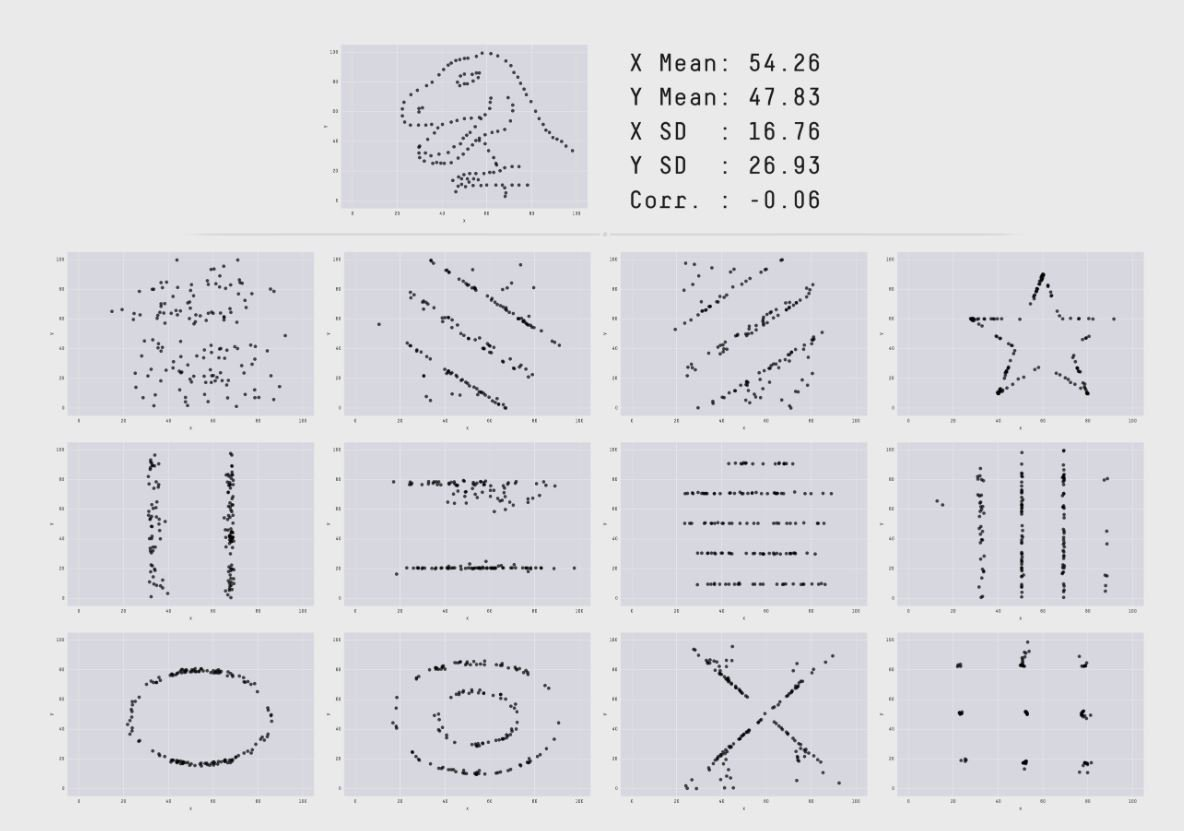
\includegraphics[width=0.7\linewidth]{./figures/matejka17fig} 

}

\caption{12 data sets created from the datasaurus by
simulated annealing. Each is restrained to the same summary statistics
but given shapes with visual peculiarity to mutate into
\autocite{matejka_same_2017}.}\label{fig:matejka17fig}
\end{figure}

It is clear that data-space visualization is needed but it becomes
complex as data dimensionality increases. Embedding (or projecting)
\(p-\)dimensional data on to a lower, \(d\)-dimensional subspace is a
common dimension reduction approach to visualize multivariate data
spaces. Traditionally a single static projection is used to summarize a
space, which necessarily shows a subset of the variation of the data.
\textcite{asimov_grand_1985} suggested the use of viewing projections
dynamically across a changing projection basis allows for more variation
to be contained and viewed temporally. This dynamic view of many
changing projections is known as \emph{tours}. While, there are
different methods of generating tour paths, human-in-the-loop
user-controlled steering (UCS) offers the finest control for navigating
the local structure.

Tours are typically viewed from standard 2D monitors, and most commonly
viewed as a projection down to 2D. A notable exception being
\textcite{nelson_xgobi_1998}, where 3D embeddings were viewed in 3D
head-tracked VR. Data visualization studies generally show benefits in
3D visuals over 2D, especially when adequate depth cues are provided.
The state of modern hardware has made VR more affordable and available
to wider audiences, at ever increasing resolutions of display than
previously possible. It is therefore timely for research to be conducted
to compare the structure and speed of comprehension of dynamic linear
projections across 2- and 3D display devices.

\section{Research objectives}\label{research-objectives}

Data and models are typically high-dimensional, with many variables and
parameters. Developing new methods to visualize high dimensions has been
a pursuit of statisticians, computer scientists and visualization
researchers for decades. As technology evolves examining, extending, and
assessing current techniques, in new environments, for new data
challenges, is an important endeavor. The primary objectives of this
Ph.D.~research can then be summarized as the following.

\textbf{Research objectives (RO):}

\begin{enumerate}
\def\labelenumi{\arabic{enumi}.}
\item
  \textbf{How can UCS be generalized to work within graphic-specific
  environments for 2D projections?}\\
  (Work in progress, chapter \ref{ch:workinprogress}.)\\
  Building from the UCS algorithm in \textcite{cook_manual_1997}, the
  algorithm should be modified for generalized use with graphic-specific
  environments. This enables fine control to explore the sensitivity of
  structure to the variable contributing to the projection and sets the
  foundation to be used in the remaining objectives.
\item
  \textbf{Does 2D UCS tours provide benefits over alternatives?}\\
  (Future work, chapter \ref{ch:future_work}.)\\
  The quality and effectiveness of 2D UCS will be compared with
  alternatives of static, single, linear and non-linear projection
  techniques. They will be quantified by the measurement of structure,
  variation, and clustering across on benchmark datasets.
\item
  \textbf{How can UCS be extended to 3D?}\\
  (Future work, chapter \ref{ch:future_work}.)\\
  The addition of a 3rd dimension potentially allows for the improved
  perception of the structure of the data in dynamic UCS. To investigate
  this UCS algorithm needs to be extended to a third dimension. This
  would also allow for novel application multi-parameter function
  projection. This will involve the addition of a new angle and it
  controls to the projection space, reference axes, and manipulation
  space. In particular, the manipulation space, now in 4D, will be hard
  to visualize, but it should be able to stand as a mathematical
  construct facilitated through interaction with a point (the projection
  coefficients of the selected manipulation variable) on the now 3D
  reference axes volume.
\item
  \textbf{Does UCS in 3D displays provide benefits over 2D displays?}\\
  (Future work, chapter \ref{ch:future_work}.)\\
  The addition of a 3rd dimension has previously been shown to provide
  benefits. The extension of UCS into 3D should be used to explore the
  potential benefits of UCS projections as well. Interactive,
  time-varying tours theoretically allow for improved understanding and
  comprehension speed of the structure of the data. These metrics will
  be measured across the display device (including a 2D standard
  monitor, 3D head tracked monitor, and 3D head-mounted display).
\end{enumerate}

\textbf{Contributions:}

The intended contributions and scope of this research can be summarized
as:

\begin{enumerate}
\def\labelenumi{\arabic{enumi}.}
\tightlist
\item
  A modified UCS algorithm and new implementation applied to
  contemporary high energy physics and astrophysics applications in 2D
  animation frameworks.
\item
  A performance comparison of static and interactive UCS projection
  techniques assessed on benchmark data sets from the recent literature.
\item
  A new algorithm for UCS in 3D. With new applications to function
  visualization in 3D.
\item
  Quantitative understanding of the relative benefits of UCS across 2-
  and 3D display devices.
\end{enumerate}

\section{Methodology}\label{methodology}

This research is interdisciplinary; it stems from a linear dimension
reduction technique developed by statisticians and extended with
information technology into 3D including VR technologies, with
applications in high energy physics
identified\autocite{cook_dynamical_2018}. Experts in these fields
correspondingly supervise the research.

The research corresponding with RO \#1 entails a work in progress
\textbf{algorithm design} following the work in
\textcite{cook_manual_1997}. The proposed algorithm discusses the
generalized application of UCS for use across animation-specific
frameworks. The outcome of this is an \emph{R} package,
\texttt{spinifex}, which will be submitted to CRAN and for hosting and
distribution. This forms the foundation for future work in the remaining
objectives.

The second objective is addressed with a benchmark dataset
\textbf{performance comparison} between dynamic linear projections and
alternatives (static linear and static non-linear projections such as
principal component analysis, multi-dimensional scaling, and
t-distributed neighbor embeddings, described in more detail in chapter
\ref{ch:future_work}). Benchmark datasets will be compared across
techniques, measurements will include variation explained, transparency
to the original variable space, clustering identification, and outlier
identification.

The research for RO \#3 involves \textbf{algorithm design}, where the
work in RO \#1 will be extended to display with the use of a third
spatial dimension. Surface and function projections will also be
developed. This forms the calculation base for the work. Several
difficulties may arise when bringing dynamic projection into 3D spaces,
especially when exploring 3D surfaces (discussed in more detail in
chapter \ref{ch:future_work}).

The research resulting from RO \#4 is a controlled \textbf{usability
study} to explore the efficacy of bringing UCS into 3D as compared
across various display devices, in a standardized interface allowed by
the work stemming from RO \# 3. In this design, the factors are user
tasks (such as separation of clusters and ranking of manipulation
variable) across the treatment of display device (including 2D standard
monitor, 3D head-tracked monitor, and head-mounted display).
Quantitative measurements include participant speed and accuracy of
tasks, biometric readings, and subjective Likert surveys of
participants. A lineup-type model as outlined in
\textcite{hofmann_graphical_2012} may also be employed for assessing the
quality of display types.

\section{Workflow and
reproducibility}\label{workflow-and-reproducibility}

Figure \ref{fig:dataanalysisworkflow} depicts the general data analysis
workflow \autocite{wickham_r_2016}. Where data first must be imported
into a tool, the structure of the data must be tidied and ordered neatly
into the correct use format. After the data enters a repeating cycle,
where values may be transformed, visualized, and modeled with
communication going to the appropriate recipients. The research proposed
in this document aids exploratory data analysis as well as the
visualization aspect of this workflow. Mature analysis workflow is also
made reproducible with the use of programmatic scripts.





\begin{figure}

{\centering 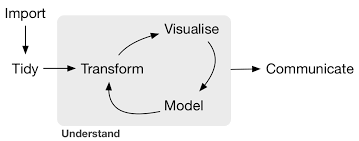
\includegraphics[width=1\linewidth]{./figures/data_analysis_workflow} 

}

\caption{Data analysis workflow
\autocite{wickham_r_2016}. This research aids visualization in
exploratory data analysis and workflow.}\label{fig:dataanalysisworkflow}
\end{figure}

The programing language, \emph{R}, is used in the work described below
to import, tidy, and transform data. It can be used directly to
visualize 2D tours (RO \#1 \& 2) or be consumed into the game engine
\emph{Unity} to visualize 3D tours (RO \#3 \& 4). Doing analysis and
writeup in such programmatic ways allow work to be done reproducibly.
Where data, analysis, and code are stored in the same directory.
Reproducible work facilitates validation, maintains transparency and
minimizes the chance for human error. Reproduction of work is a key
feature to validate and defend the claims and methodology held within a
work. Directories of current and planned work are/will be hosted
publicly on GitHub, including this report. Accessing the source files
for this report is discussed in section \ref{sec:source}.

\section{Project overview}\label{ch:projectoverview}

Figure \ref{fig:ProjectOverview} depicts a schematic flow chart that the
research objectives will be executed in. The research stemming from RO
\#1, the application of 2D user-controlled steering (UCS), sets the
foundation for which the other objectives can be researched. RO \#3, the
application of 3D UCS, must precede RO \#4, as it explores the efficacy
of 3D UCS across display devices. RO \#2, the comparison of 2D UCS vs
alternatives, must come after RO \#1, but is of lower priority to RO \#3
\& 4, and so will be conducted last, in the event of a time crunch.




\begin{figure}

{\centering 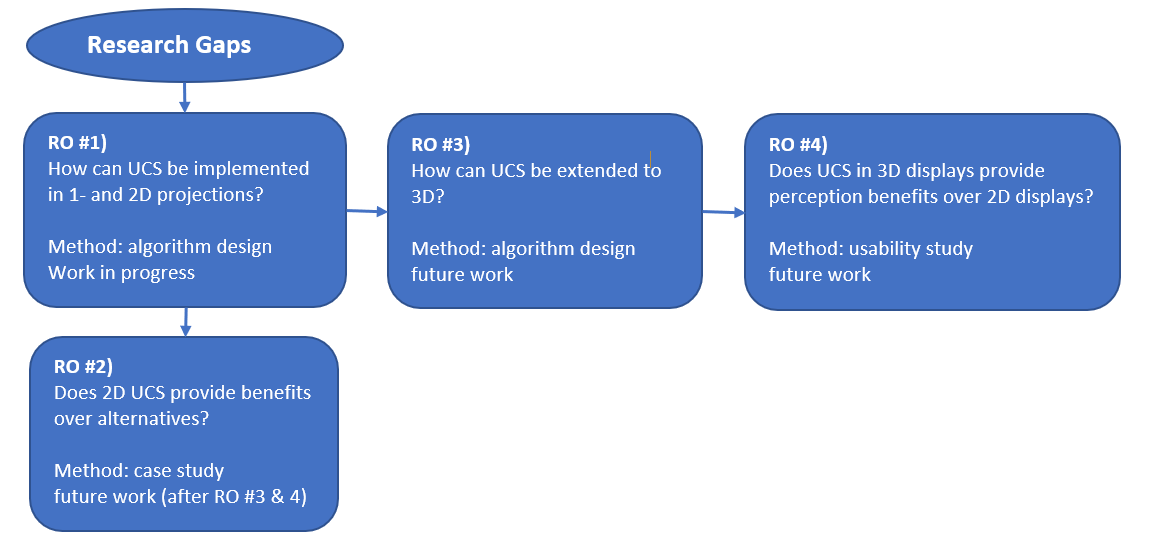
\includegraphics[width=1\linewidth]{./figures/ProjectOverview} 

}

\caption{Flow chart of research objective dependencies,
work order, and methodology.}\label{fig:ProjectOverview}
\end{figure}

In this report, the related literature is discussed in chapter
\ref{ch:lit_review}. A brief overview of the research is given in
chapter \ref{ch:projectoverview}, followed by ongoing work and future
work in chapters \ref{ch:workinprogress} and \ref{ch:future_work}
respectively. A prospective timeline is listed in chapter
\ref{ch:timeline}. Notation for dynamic projections and VR data
visualization can be found in appendix \ref{ch:glossary} and an excerpt
of a paper to be submitted to the R Journal can be found in appendix
\ref{ch:spinifex}.

\chapter{Literature review}\label{ch:lit_review}

The following chapter discusses the current research in two primary
areas: dynamic linear projections (collectively known as tours) and
multivariate data visualization in stereoscopic 3D. After each section,
research gaps are highlighted.

\section{Dynamic linear projections of multivariate data
(tours)}\label{sec:tour}

\subsection{Overview}\label{overview}

The introduction established that visualizing data-space is an important
aspect of exploratory data analysis and data analysis in general. Yet,
there is an inherent difficulty as the dimensionality of data increases.
In univariate data sets histograms or smoothed density curves are
employed to visualize data. In bivariate data, \(XY\) scatterplots and
contour plots (2D density) can be employed. In three dimensions, the two
most common techniques are 3D
scatterplot\footnote{Graphs depicting three dimensions are typically viewed on a 2D display, in print or with a standard monitor. These are 2D images of monocular 3D spaces, sometimes referred to as 2.5D data visualization, more on this in section \ref{sec:3d-terminology}.}
or 2D scatterplot with the 3rd variable as an aesthetic (such as color,
size, or height). These aesthetic cues convey some information but are
not a sufficient replacement for axes for use with continuous variables.

As dimensionality of the data, \(p\), increases the visualization of
data-space quickly becomes complex. It is common that visualizing
data-space is dropped in favor of graphing model-space (for example
residuals), parameter-space (in fewer dimensions), or worse yet: long
tables of statistics without visuals
\autocite{wickham_visualizing_2015}. To preserve the visualization of
data-space, a solution that scales with the dimensionality of data is
needed; this is where dimensionality reduction comes in. This work will
focus on a group of dynamic linear projection techniques collectively
known as \emph{tours}. The scope of the project lies within the dynamic
linear projections; a broader review of dimensionality reduction
techniques is discussed in the review paper by
\textcite{grinstein_high-dimensional_2002}. Tours are used for a couple
of salient features: the use of linear projections maintains
transparency back to the original variable space (which non-linear
projections lose) and the use of many projections shows more variation
than a single linear projection. Employing the breadth of tours extends
the dimensionality of visualizations, and with it, the intrinsic
understanding of the structure and distribution of data that is more
succinct or beyond the reach of summary statistics alone.

Let \(p\) be the dimensionality of the data, and \(d\) be the dimension
of the projection space. Tours perform linear dimensionality reduction,
orthogonally projecting \(p\)-space down to \(d(\leq p)\) dimensions.
Many such projections are interpolated, each making small rotations in
\(p\)-space. These frames are then viewed in order as an animation of
the lower dimensional embedding changing as the original variable space
is manipulated. Shadow puppets offer a useful analogy to aid in
conceptualizing tours. Imagine a fixed light source facing a wall. When
an object is introduced it projects a 2D shadow onto the wall. This is a
physical representation of a simple projection, that from \(p=3\) down
to \(d=2\). If the object rotates then the shadow correspondingly
changes. Observers watching only the shadow are functionally watching a
2D tour as the 3D object is manipulated. Some orientations explain more
information about the shape of the object than others while watching an
animation of the shadow changing gives a more robust understanding than
looking at any one frame. More complex structures generally require more
time to comprehend the nature of the geometry. These features hold for
tours as well.

\emph{An extended tour notation is listed in the appendix section
\ref{sec:tour_notation}.}

\subsection{History}\label{history}

The first tour was introduced was the \emph{grand tour} in
\textcite{asimov_grand_1985} at the Stanford Linear Accelerator,
Stanford University. Asimov suggested three types of grand tours: torus,
at-random, and random-walk. The original application of tours was
performed on high energy physics on the PRIM-9 system.

Before choosing projection paths randomly, an exhaustive search of
\(p-\)space was suggested by \textcite{mcdonald_interactive_1982}, also
at the Stanford Linear Accelerator. This was later coined \emph{little
tour}.

\textcite{friedman_projection_1974} and later
\textcite{huber_projection_1985} recommended projection pursuit (also
referred to as PP). Projection pursuit optimizes an objective function
before it removes a single component/variable and then iterates in this
newly embedded subspace. Within each subspace, the projection seeks for
a local extremum via a hill climbing algorithm on an objective function.
This formed the basis for \emph{guided tours} suggested by
\textcite{hurley_analyzing_1990}.

The grand and little tours have no input from the user aside from the
starting basis. Guided tours allow for an index to be selected. The bulk
of tour development since has largely been around the dynamic display,
user interaction, geometric representation, and application.

\subsection{Path generation}\label{sec:path_generation}

A fundamental aspect of tours is the path of rotation. There are four
primary distinctions of tour path generation
\autocite{buja_computational_2005}: random choice, data-driven,
precomputed choice, and manual control.

\begin{itemize}
\tightlist
\item
  Random choice, \emph{grand tour}, constrained random walks
  \(p\)-space. Paths are constrained for changes in direction small
  enough to maintain continuity and aid in user comprehension

  \begin{itemize}
  \tightlist
  \item
    torus-surface \autocite{asimov_grand_1985}
  \item
    at-random \autocite{asimov_grand_1985}
  \item
    random-walk \autocite{asimov_grand_1985}
  \item
    \emph{local tour} \autocite{wickham_tourr_2011}, a sort of grand
    tour on a leash, such that it goes to a nearby random projection
    before returning to the original position and iterating to a new
    nearby projection.
  \end{itemize}
\item
  Data-driven, \emph{guided tour}, optimizing some objective
  function/index within the projection-space, called projection pursuit
  (PP) \autocite{hurley_analyzing_1990}, including the following
  indexes:

  \begin{itemize}
  \tightlist
  \item
    holes \autocite{cook_projection_1993} - moves points away from the
    center.
  \item
    cmass \autocite{cook_projection_1993} - moves points toward the
    center.
  \item
    lda \autocite{lee_projection_2005} - linear discriminant analysis,
    seeks a projection where 2 or more classes are most separated.
  \item
    pda \autocite{lee_projection_2010} - penalized discriminant analysis
    for use in highly correlated variables when classification is
    needed.
  \item
    convex \autocite{laa_using_2019} - the ratio of the area of convex
    and alpha hulls.
  \item
    skinny \autocite{laa_using_2019} - the ratio of the perimeter
    distance to the area of the alpha hull.
  \item
    stringy \autocite{laa_using_2019} - based on the minimum spanning
    tree (MST), the diameter of the MST over the length of the MST.
  \item
    dcor2D \autocites{grimm_mbgraphic:_2017}{laa_using_2019} - distance
    correlation that finds linear and non-linear dependencies between
    variables.
  \item
    splines2D \autocites{grimm_mbgraphic:_2017}{laa_using_2019} -
    measure of non-linear dependence by fitting spline models.
  \item
    other user-defined objective indices can be applied to the framework
    provided in the \emph{tourr} package \textcite{wickham_tourr_2011}.
  \item
    Another data-drive tour is the \emph{dependence tour}, a combination
    of \(n\) independent 1D tours. A vector describes the axis each
    variable will be displayed on. for example \(c(1, 1, 2, 2)\) is a 4-
    to 2D tour with the first 2 variables on the first axis, and the
    remaining on the second.

    \begin{itemize}
    \tightlist
    \item
      \emph{correlation tour} \autocite{buja_data_1987}, a special case
      of the dependence tour, analogous to canonical correlation
      analysis.
    \end{itemize}
  \end{itemize}
\item
  Precomputed choice, \emph{planned tour}, in which the path has already
  been generated or defined.

  \begin{itemize}
  \tightlist
  \item
    \emph{little tour} \autocite{mcdonald_interactive_1982}, where every
    permutation of variables is stepped through in order, analogous to
    brute-force or exhaustive search.
  \item
    a saved path of any other tour, typically an array of basis targets
    to interpolate between.
  \end{itemize}
\item
  Manual control, \emph{manual tour}, a constrained rotation on selected
  manipulation variable and magnitude \autocite{cook_manual_1997}.
  Typically used to explore the local area after identifying an
  interesting feature, perhaps via guided tour.
\end{itemize}

\subsection{Path evaluation}\label{path-evaluation}

Consider projection down to 2D, then each projection is called a 2-frame
(each spanning a 2-plane). Mathematically, a Grassmannian is the set of
all possible unoriented 2-frames in \(p\)-space, \(\textbf{Gr}(2,~p)\).
\textcite{asimov_grand_1985} pointed out that the unique 2-frames of the
grand tour approaches \(\textbf{Gr}(2,~p)\) as time goes to infinity.
The \emph{density} of a tour is defined as the fraction of the
Grassmannian explored. Ideally, an exploring tour will be dense, but the
time taken to become dense vastly increases as variable space increases
dimensionality. \emph{Rapidity} is then defined as how quickly a tour
encompasses the Grassmannian. Due to the random selection of a grand
tour, it will end up visiting homomorphisms of previous 2-frames before
all unique values are visited, leading sub-optimal rapidity.

The little tour introduced in \textcite{mcdonald_interactive_1982}, on
the other hand, is necessarily both dense and rapid, performing
essentially an exhaustive search on the Grassmannian. However, this path
uninteresting and with long periods of similar projections strung
together. The Grassmannian is necessarily large and increases
exponentially at the rate of \(p\). Viewing of the whole Grassmannian is
time-consuming, and interesting projections are sparse, there was a
clear space for computers to narrow the search space.

Guided tours \autocite{hurley_analyzing_1990} optimize an objective
function generating path will be a relatively small subset of the
Grassmannian. As they are not used for exploration, density and rapidity
are poor measures. On the other hand, they excel at finding interesting
projections quickly. Recently, \textcite{laa_using_2019}, compared
projection pursuit indices with the metrics: \emph{smoothness,
squintability, flexibility, rotation invariance} and \emph{speed}.

\subsection{Geometric display by dimensionality}\label{sec:geom_display}

Up to this point, 2D scatterplots have been the primary display
discussed, they offer a logical display for viewing embeddings of
high-dimensional point clouds. However, other geometrics offer perfectly
valid projections as well.

\begin{itemize}
\tightlist
\item
  1D geometrics (geoms)

  \begin{itemize}
  \tightlist
  \item
    1D densities: such as histogram, average shifted histograms
    \autocite{scott_averaged_1985}, and kernel density
    \autocite{scott_incorporating_1995}.
  \item
    image (pixel): \autocite{wegman_pixel_2001}.
  \item
    time series: where multivariate values are independently lagged to
    view peak and trough alignment. Use case is discussed in
    \autocite{cook_manual_1997}.
  \end{itemize}
\item
  2D geoms

  \begin{itemize}
  \tightlist
  \item
    2D density (available on GitHub at
    \url{https://github.com/nspyrison/tourr})
  \item
    \(XY\) scatterplot
  \end{itemize}
\item
  3D geoms

  \begin{itemize}
  \tightlist
  \item
    Anaglyphs, sometimes called stereo, where red images are positioned
    for the left channel and cyan for the right when viewed with
    corresponding filter glasses give a perception of depth to the
    image.
  \item
    Depth, which gives depth cues via aesthetic mappings, most common
    size and/or color of data points.
  \end{itemize}
\item
  \(d\)-dimensional geoms

  \begin{itemize}
  \tightlist
  \item
    Andrews curves \autocite{andrews_plots_1972}, smoothed variant of
    parallel coordinate plots, discussed below.
  \item
    Chernoff faces \autocite{chernoff_use_1973}, variables linked to the
    size of facial features. The idea is to apply the human
    facial-perception for rapid, cursory, like-ness comparisons between
    observations.
  \item
    Parallel coordinate plots {[}\textcite{ocagne_coordonnees_1885};
    wegman\_hyperdimensional\_1990{]}, where any number of variables are
    plotted in parallel with observations linked to their corresponding
    variable value by polylines.
  \item
    Scatterplot matrix (SPLOM) \autocite{chambers_graphical_1983},
    showing a triangle matrix of bivariate scatterplots with 1D density
    on the diagonal.
  \item
    Radial glyphs, radial variants of parallel coordinates including
    radar, spider \autocite{duffin_spiders:_1994}, and star glyphs
    \autocite{siegel_surgical_1972}.
  \end{itemize}
\end{itemize}

\subsection{Tour software}\label{tour-software}

Tours have yet to be widely adopted, due in part, to the fact that print
and static .pdf output does not accommodate dynamic viewing. Conceptual
abstraction and technically density have also hampered user growth. Due
to low levels of adoption and the rapid advancement of technology
support and maintenance of such implementations give them a particularly
short life span. Despite the small user base, there have been a fair
number of tour implementations, including:

\begin{itemize}
\tightlist
\item
  spinifex
  \href{https://github.com/nspyrison/spinifex}{github.com/nspyrison/spinifex}
  -- R package, all platforms.
\item
  tourr \autocite{wickham_tourr_2011} -- R package, all platforms.
\item
  CyrstalVision \autocite{wegman_visual_2003} -- for Windows.
\item
  GGobi \autocite{swayne_ggobi:_2003} -- for Linux and Windows.
\item
  DAVIS \autocite{huh_davis:_2002} -- Java based, with GUI.
\item
  ORCA \autocite{sutherland_orca:_2000} -- Extensible toolkit build in
  Java.
\item
  VRGobi \autocite{nelson_xgobi_1998} -- for use with the C2, tours in
  stereoscopic 3D displays.
\item
  ExplorN \autocite{carr_explorn:_1996} -- for SGI Unix.
\item
  ExploRe \autocite{hardle_xplore:_1995}
\item
  XGobi \autocite{swayne_xgobi:_1991} -- for Linux, Unix, and Windows
  (via emulation).
\item
  XLispStat \autocite{tierney_lisp-stat:_1990} -- for Unix and Windows.
\item
  Explor4 \autocite{carr_explor4:_1988} -- Four-dimensional data using
  stereo-ray glyphs.
\item
  Prim-9 \autocites{asimov_grand_1985}{fisherkeller_prim-9:_1974} -- on
  an internal operating system.
\end{itemize}

\subsection{Research gaps}\label{research-gaps}

Dynamic projections offering UCS have not incorporated recent animation
frameworks (\textbf{RO \#1}). This leaves the class of dynamic linear
projections without the most precise, fine-scale control of rotating
\(p\)-space. This should be implemented with an eye on extensibility and
maintainability.

A comparative study outlining the benefits of UCS vs alternatives is
also absent from the literature (\textbf{RO \#2}). The benefits of
dynamic linear projections hold in theory, but a direct comparison with
popular alternatives should be made. Barriers to adoption and sharing
should also be kept in mind as the dynamic display is not easy to
display on print and in .pdf documents.

\section{Multivariate data visualization in 3D}\label{sec:3d}

The scope of this research pertains to numeric multivariate data, a
wider overview of 3D data visualization is discussed in chapter 2 of
\textcite{marriott_immersive_2018}. Terminology for 3D visuals is in the
glossary section \ref{sec:3d-terminology}.

\subsection{A rocky start}\label{a-rocky-start}

Scientific visualization has readily adopted mixed realities as a large
amount of the science exists in three spatial dimensions, lending itself
well to virtual immersion \autocite{marriott_immersive_2018}. Data
visualization, on the other hand, has been slow to utilize graphics
above 2.5D, (and haptic interaction) primarily due to the mixed results
of over-hyped of 3D visuals from the 1980s and '90s
\autocite{munzner_visualization_2014}. Since then, however, there have
been several promising studies suggesting that it is time for data
visualization to revisit and adopt the use of 3D visuals for specific
combinations of displays and depth cues.

\subsection{3D rotated projections vs 3 2D orthogonal
projections}\label{d-rotated-projections-vs-3-2d-orthogonal-projections}

Three orthogonal 2D views can represent the three face-on views of 3D
shapes. When 3D representations are used with binocular cues, they are
found to have more accurate perception than 2D counterparts
\autocite{lee_effects_1986}.

Between 3D and split view 2D of three-dimensional economics, data
\textcite{wickens_implications_1994} asked participants questions
integrating several variables, finding that 3D visuals resulted in
faster answers when questions involved three dimensions, while the speed
was similar when questions involved fewer dimensions.

Using 3D rotated projections gives more precise (relative to 2D)
estimates of the height a ball is suspended above complex box shapes,
while combinations of 2D and 3D give the most precise orientation and
positioning information \autocite[depicted in figure
\ref{fig:tory06fig}]{tory_visualization_2006}.








\begin{figure}

{\centering 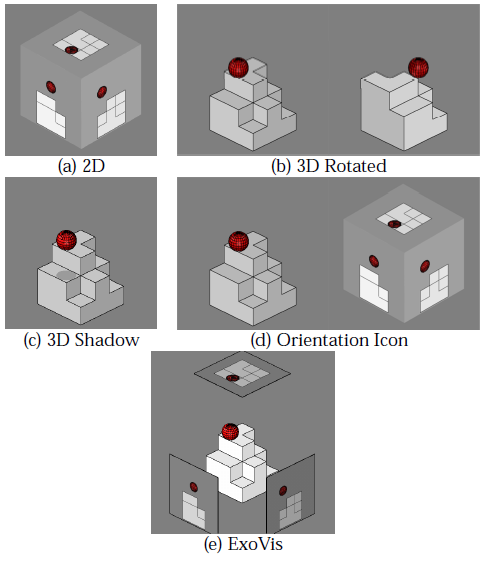
\includegraphics[width=0.5\linewidth]{./figures/tory06fig} 

}

\caption{Screen capture from
\textcite{tory_visualization_2006}: ``fig. 1 (a) 2D, (b) 3D Rotated, (c)
3D Shadow, (d) Orientation Icon, and (e) ExoVis displays used in
Experiment 1 (position estimation). Participants estimated the height of
the ball relative to the block shape. In this example, the ball is at
height 1.5 diameters above the block shape.''}\label{fig:tory06fig}
\end{figure}

\textcite{sedlmair_empirical_2013}, depicted in figure
\ref{fig:sedlmair13fig}, asked users about cluster separation across 2D
scatterplots, 2D scatterplot matrices (SPLOMs) and interactive 3D
scatterplots, PCA (linear projection), and t-SNE (non-linear projection)
as viewed in monocular 3D from a standard monitor. They conclude that
interactive 3D scatterplots perform worse for class separation. This
result is surprising as the extra dimension theoretically allows for the
clustering structure to be seen and explored more clearly.














\begin{figure}

{\centering 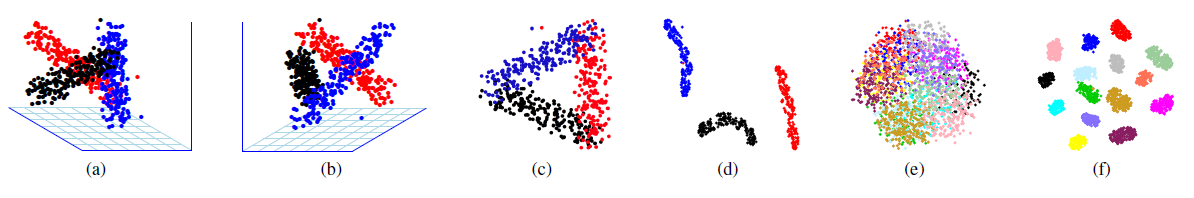
\includegraphics[width=1\linewidth]{./figures/sedlmair13fig} 

}

\caption{Screen capture of ``figure 5. example of a mesh
display'' from \textcite{sedlmair_empirical_2013}: ``fig. 5. (a)-(d):
Screenshots of the entangled dataset \texttt{entangled1-3d-3cl-separate}
designed to show the most possible benefits for i3D. (a),(b) two
viewpoints of the same i3D PCA scatterplot. An accompanying video shows
the full 3D rotation. (c) 2D PCA projection. (d) t-SNE untangles this
class structure in 2D. (e)-(f): 2D scatterplots of the reduced
\texttt{entangled2-15d-adjacent} dataset which we designed to have a
ground truth entangled class structure in 15D. (e) Glimmer MDS cannot
untangle the classes, neither can PCA and robPCA (see supplemental
material). (f) t-SNE nicely untangles and separates the ground truth
classes in 2D.''}\label{fig:sedlmair13fig}
\end{figure}

\subsection{Comparing 3D and 2D embeddings of multivariate
data}\label{comparing-3d-and-2d-embeddings-of-multivariate-data}

\textcite{nelson_xgobi_1998}, depicted in figure \ref{fig:nelson98fig},
had \(n=15\) participants perform brushing and identification tasks (of
clusters, structure, and data dimensionality) in 3D with head-tracked
binocular VR. 3D proved to have a substantial advantage for cluster
identification and some advantage in identifying the shape. Brushing did
take longer in VR, perhaps due to the lower familiarity of manipulating
3D spaces.







\begin{figure}

{\centering 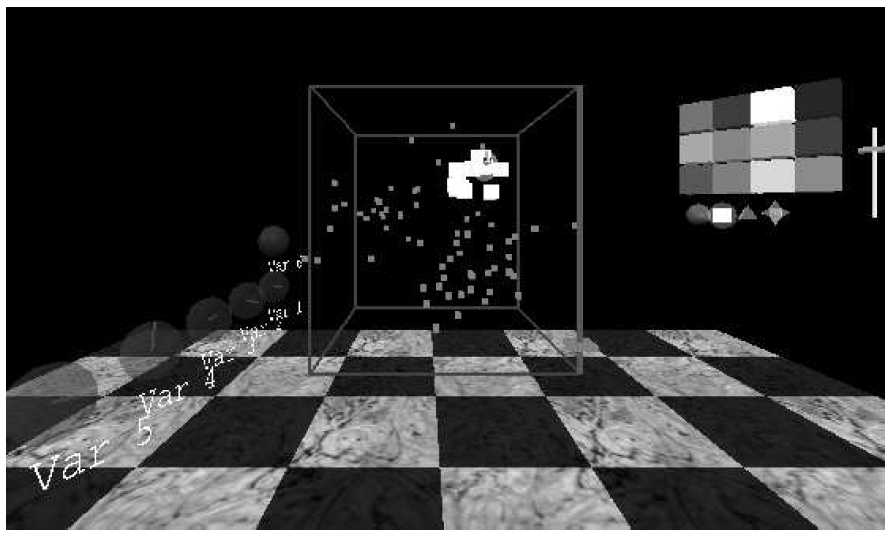
\includegraphics[width=0.7\linewidth]{./figures/nelson98fig} 

}

\caption{Screen capture from \textcite{nelson_xgobi_1998}:
``figure 4: This is a picture of a 3-D room, running VRGobi. Data is
plotted in the center, with painting tools to the right and variable
spheres to the left. In the viewing box, the data can be seen to contain
three clusters, and one is being brushed.''}\label{fig:nelson98fig}
\end{figure}

Another study, \textcite{gracia_new_2016} performed dimensionality
reduction down to 2- and 3D scatterplots, both displayed in monocular 3D
on a standard monitor. Users were found to more accurately compare
distances between points and identify outliers on 3D scatterplots.
However, both tasks were performed slower with the use of the 3D
scatterplots and statistical significance was not reported.

\textcite{wagner_filho_immersive_2018}, depicted in figure
\ref{fig:wagner18fig}, performed an \(n=30\) empirical study on PCA
embedded projections, measuring perception error across 4 tasks and 3
display types: 2D, static 3D, and immersive 3D. Overall task error was
less in static and immersive 3D relative to 2D. According to the user
Likert-scale survey, 2D is slightly easier to navigate and slightly more
comfortable, while, static and immersive 3D displays are slightly easier
to interact with and moderately easier to find information on.





\begin{figure}

{\centering 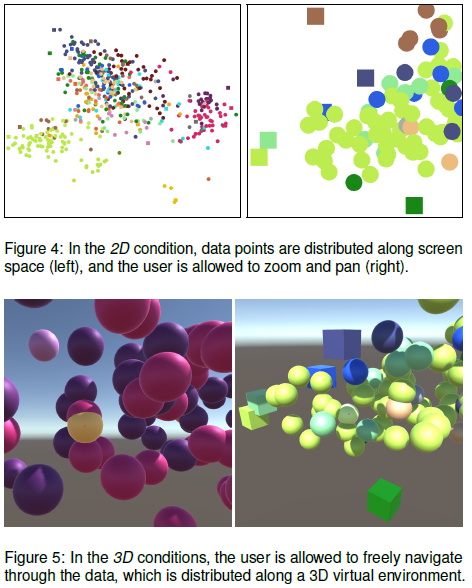
\includegraphics[width=0.5\linewidth]{./figures/wagner18fig} 

}

\caption{Screen capture from
\textcite{wagner_filho_immersive_2018}, original captions contained in
the capture.}\label{fig:wagner18fig}
\end{figure}

\subsection{Immersive analytics platform in
VR}\label{immersive-analytics-platform-in-vr}

Immersive analytics is an emerging field, where data visualization and
analysis is facilitated in an intuitive, immersive virtual reality
environment \autocites{chandler_immersive_2015}{cordeil_immersive_2017}.
An example of which is shown in \textcite{cordeil_imaxes:_2017}
introduces a collaborative space for immersive data analysis. Where axes
are displayed and intuitively interacted with while responding to
proximity to other variable axes and popping into place changing the
resulting geometric display. For example, three variables can be placed
as the \(x,~y,~z-\) axes for a 3D scatterplot or stood up right next to
each other for a parallel coordinate plot. The subsequent work in
\textcite{cordeil_immersive_2019} builds from the previous reference and
refines it for the next iteration in interactive, scalable data
visualization in virtual spaces.




\begin{figure}

{\centering 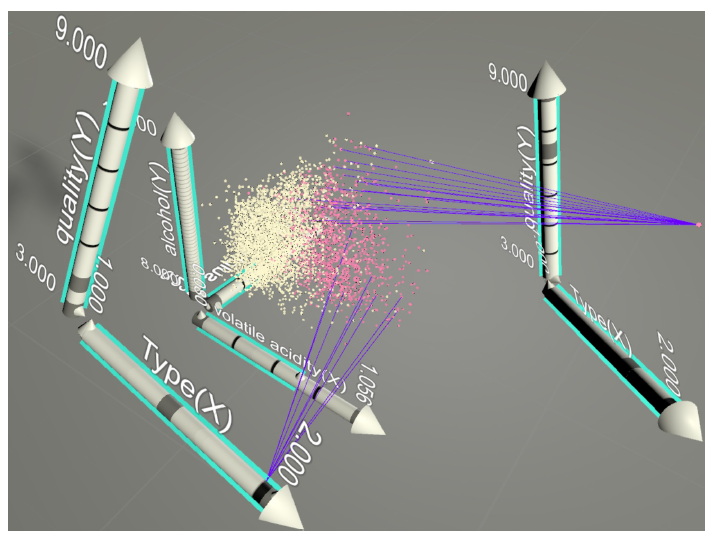
\includegraphics[width=0.5\linewidth]{./figures/cordeil2017fig} 

}

\caption{Screen capture of figure 15 from
\textcite{cordeil_imaxes:_2017}.}\label{fig:cordeil2017fig}
\end{figure}

\subsection{Research gaps}\label{research-gaps-1}

When comparing between 2- and 3D orthogonal views, in general, studies
show that perception accuracy is better in 3D, though manipulation speed
is generally slower. The speed discrepancy is confounded by the
difference in users familiar with manipulating 2D vs 3D spaces
\autocites{lee_effects_1986}{wickens_implications_1994}{tory_visualization_2006}[counterexample][]{sedlmair_empirical_2013}.

Similar results have been shown in static, 3D projected spaces
\autocites{gracia_new_2016}{wagner_filho_immersive_2018} and in dynamic
2D embedded spaces depicted in immersive 3D
\autocite{nelson_xgobi_1998}. Modern VR hardware brings about a steady
improvements to quality, resolution while driving down cost, making VR
more easily accessible than ever. It's timely to review dynamic 3D
projections and do so in immersive spaces to quantify the corresponding
benefits (\textbf{RO \#3 \& 4}).

\chapter{Work in progress}\label{ch:workinprogress}

Extending the algorithm for UCS in 2D for generalized use in graphics
environments is fundamental to the extension of the UCS into 3D space.
This forms the foundation for future work addressed in the remaining
research objectives. This is a synthesis of the work that will be
submitted to the R Journal. A wider discussion of implementation as an
\emph{R} package and application to high energy physics data
\autocites{wang_visualizing_2018}{cook_dynamical_2018} is attached in
appendix \ref{ch:spinifex} formatted as a paper.

\section{RO \#1) How can UCS be generalized to work within
graphic-specific environments for 2D
projections?}\label{ro-1-how-can-ucs-be-generalized-to-work-within-graphic-specific-environments-for-2d-projections}

This chapter builds off of \emph{manual tours}
\autocite{cook_manual_1997} and modifies the algorithm for generalized
use in graphics implementations. Manual tours allow users to rotate a
selected variable into and out of a 2D projection of high-dimensional
space for user-controlled steering (UCS). The primary use is to
determine the sensitivity of the structure to the contributions of a
selected manipulation variable. This is particularly useful once a
feature of interest has been identified, for example, by a guided tour.

\section{Algorithm}\label{sec:wip_algorithm}

The algorithm for generating a manual tour path involves these steps:

\begin{enumerate}
\def\labelenumi{\arabic{enumi}.}
\tightlist
\item
  Given a 2D projection basis, choose a variable to explore. This is
  called the ``manip'' variable.
\item
  Create a 3D manipulation space, where the manip variable has a full
  contribution.
\item
  Generate a rotation sequence which zeros coefficient and increases it
  to 1 before returning to the initial position.
\end{enumerate}

\subsection{Step 1 Choose variable of
interest}\label{step-1-choose-variable-of-interest}

Start with multivariate data in an \(n \times p\) numeric matrix, and an
orthonormal (orthogonal and each column normalized to have a norm of 1)
\(p \times d\) basis set is describing the projection from \(p-\) to
\(d-\)space. Select a manipulation (manip) variable. The coefficients of
this variable will be operated on.

\subsection{Step 2 Create the manip
space}\label{step-2-create-the-manip-space}

A fully 3D space is created, using the Gram-Schmidt process, within
which to rotate the manip variable into and out of the projection plane.
The new dimension giving the basis the freedom to rotate `out-of-plane',
akin to being able to lift a piece of paper, rather than being confined
to the top of a table.

\subsection{Step 3 Generate rotation}\label{step-3-generate-rotation}

generate an animation sequence of 2D projection matrices that fully
rotates the manip variable into and out of the projection. The sequence
can be passed to any graphics rendering to display the projected data.

\section{Display projection sequence}\label{display-projection-sequence}

A 2D projection of the 3D manip space is generated by multiplying the
data matrix by a projection matrix. The algorithm needs only one copy of
the data, and the sequence of projection matrices, to generate the data
animation. The 2D projected data is currently displayed as a
scatterplot, but alternative choices like a contour plot of the
bivariate density could be easily substituted.

\chapter{Future work}\label{ch:future_work}

\section{RO \#2) Does 2D UCS provide benefits over
alternatives?}\label{ro-2-does-2d-ucs-provide-benefits-over-alternatives}

Dimensionality reduction is important to viewing high dimensional data
spaces. There are various techniques have been developed to view
projections of data. The research answering this question would quantify
the potential benefits of dynamic 2D UCS over commonly used
alternatives. All comparison groups would be unsupervised (agnostic of
clustering), static, single embeddings in a lower dimension, and would
include:

\begin{itemize}
\tightlist
\item
  \textbf{Principal Component Analysis (PCA)}
  \autocite{pearson_liii._1901}, a linear transformation that forms
  orthogonal linear combinations of the variables by maximizing the
  amount of variation that is independent of all preceding components.
  That is, the first principal component is the linear combination that
  explains the most variation in one direction, the second component
  explaining the most of the remaining variation and is orthogonal to
  the first, and so on.
\item
  \textbf{Multi-Dimensional Scaling (MDS)}, non-linear dimension
  reduction that compares pairwise distances between observations.
\item
  \textbf{t-distributed neighbor embeddings (tSNE)}
  \autocite{maaten_visualizing_2008}, a nonlinear technique that
  iterates epochs of 1) constructing a probability distribution for
  selecting neighboring data and 2), minimizing Kullback-Leibler
  divergence (a measure of relative entropy).
\end{itemize}

Unfortunately, static linear projections necessarily lose the variation
of the components not displayed, while non-linear techniques lose
transparency back to the original variable space. On the other hand,
dynamic linear projections keep variation in tack (at the expense of
viewing over time) and preserve transparency to variable-space.
User-controlled steering of tours allows for finer exploration local
exploration, which should be reflected in the benefits over alternative
options.

The methodology for this future work is a \textbf{performance
comparison} across technique, as assessed across contemporary benchmark
datasets. Differences in the techniques make for an uneven comparison,
but measurements will be made where applicable comparing at least
variation, clustering, and structure. The design space includes data
sets, techniques, and measures of comparison.

\section{RO \#3) How can UCS be extended to
3D?}\label{ro-3-how-can-ucs-be-extended-to-3d}

The literature has shown positive results for improved perception of 3D
graphics over 2D. The additional dimension theoretically allows for the
improved structural perception in 3D scatterplots and would allow for
the novel application of the dynamic projection of multidimensional
function spaces. The research answering RO \#1 will be extended for
these uses.

The work presented in \textcite{cordeil_imaxes:_2017} creates immersive
space for users to explore data in a virtual environment. Users can
actively create different visualization by spatial manipulation of
virtual variable-axes. Bringing dynamic projection into an environment
that offers immersive interaction could be a boon to interfacing with
something so dynamic in nature. The ability to render in 3D could also
act as a common interface that can be used across various display
devices in RO \#4.

The research addressing this objective applies \textbf{algorithm
design}, first, the \emph{R} package spinifex will be extended to 3D and
function/surface projections will be developed. After the projections
are computed, \emph{Unity} will be used to render the embeddings in 3D
VR and act as a compatible front end to be used across display devices.

Manipulating 3D spaces may not be straight forward. In section
\{sec:wip\_algorithm\} the manipulation space was in 3D, where 2 angles
defined a point that was projected back to the 2D reference frame. The
now 4D manipulation space should only be necessary for internal
mathematics, where the 3 angles spanning it, could be controlled through
manipulation of a selected variable on the now 3D reference volume.
Navigating 3D space may be very intuitive or may require a slide ruler
for each axis may offer more control. An additional concern of user
interaction is the potential for objects in peripheral vision to cause
discomfort. The angular speed of the projections should be regulated for
continuity of observation and to mitigate potentially nauseating
movement.






\begin{figure}

{\centering 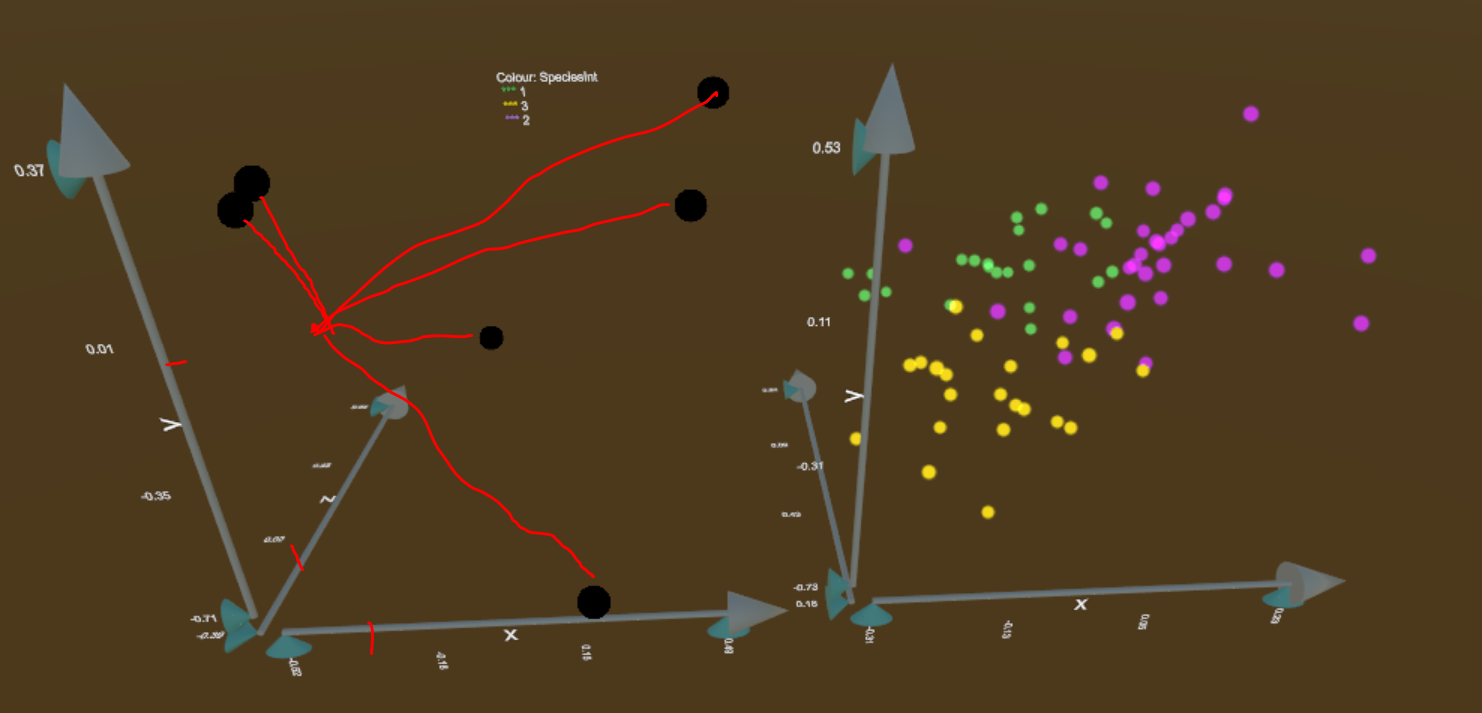
\includegraphics[width=0.7\linewidth]{./figures/RO3MockUp2} 

}

\caption{A mockup of a 3D basis reference space (left) and
scatterplot projection (right). Basis axes should extend from the origin
to allow a better perception of magnitude and direction each variable
contributes to the projection.}\label{fig:RO3MockUp}
\end{figure}

In a function projection, a multi-parameter function surface would be
projected rather than individual data points. Imagining the projection
of a unit grid is a useful middle ground. Viewing projected functions
may have several difficulties in 3D. The first is occulation, a surface
in the foreground obscures the view behind it. Opacity, wire mesh, and
projection sectioning \autocite{furnas_prosection_1994} are potential
ways to address this issue. A second issue is that it may be
disorienting or nauseating to watch surfaces folding into each other in
seemingly non-euclidean movements. Changing opacity or focus in the
vicinity of these areas may mitigate the potential concern.

The design space for this research includes the path generators
(outlined in section \ref{sec:path_generation}), geometric display
(section \ref{sec:geom_display}), layout in virtual space, dynamic
interactions. Tour paths are conceptually straight-forward mapping
between values and 3D rendering. Each geometric display will need unique
recreation, though 3D scatterplot, parallel coordinate plots, and
scatterplot matrices (SPLOMs) are currently supported in the respective
packages.

\section{RO \#4) Does UCS in 3D displays provide perception benefits
over 2D displays?}\label{UCS_3dvs2d}

The bulk of previous tours were performed in 2D, with the exceptions of
\textcite{nelson_xgobi_1998} and \textcite{arms_benefits_1999} who
conducted an \(n=15\) experimental study comparing tasks performed
across 2D and 3D tour displays. The XGobi interface was used on a
standard 2D monitor while VRGobi (on the C2 setup) was used with
head-tracked, binocular VR. The three accuracy tasks: clustering,
intrinsic data dimensionality, and radial sparseness were recorded along
with the speed of brushing data. Accuracy was the same for the
dimensionality task, while 3D display outperformed 2D on clustering, and
even more so on the radial sparsity task. However, the time taken to
brush a cluster was less than half the time in 2D displays as compared
with 3D.

\textcite{wagner_filho_immersive_2018} performed a user study on the
perception of linear projections between 2D, 3D, and immersive 3D. The
\(n=30\) user study created 3D embeddings of multidimensional data via
principal component analysis (PCA, described in RO \#2, above). Users
performed three tasks across two data sets and three displays; 2D, 3D,
and immersive 3D. Data sets were chosen to have vastly different amounts
of information contained in the 3rd principal component. They find that
the introduction of a 3rd dimension in visualization improves task
performance (perception error, task error, and completion time)
regardless of immersion for only the dataset containing large amounts of
variation in the 3rd principal component. Independent of the dataset,
immersive 3D display led to a larger subjective perception of accuracy
and engagement.

The results of \textcite{wagner_filho_immersive_2018},
\textcite{nelson_xgobi_1998} and, \textcite{arms_benefits_1999} cast
positive light on 3D spaces improving the perception of embeddings of
high-dimensional data. Others have found the same for tri-variate data.
After tours have been extended in 3D spaces (RO \#3), the effects of
viewing dynamic projections should be quantified across the display
type.

A controlled \textbf{usability study} will be performed to measure the
benefits of 3D over 2D display devices. Every participant will complete
every task on every display device. Task order and display device will
be randomly assigned to minimize learning bias. Correctness and speed of
tasks will be recorded alongside demographic data and subjective 5-point
Likert scale survey. A lineup model as outlined in
\textcite{hofmann_graphical_2012} may be employed to quantify the
``best'' display device. This lineup model is a visual variant of
statistical p-test where participants are asked to pick the real data
set as pitted against data generated from the null hypothesis. Running
such a lineup within all display devices and comparing accuracy may rank
the quality of the display device.

The factors of the study are user tasks: the perception of cluster
structure, surface structure, and ranking of manipulation variables. All
factors will be tested across the treatment of at least three display
devices: standard 2D monitor, stereoscopic 3D monitor (on a zSpace 200),
and head-mounted VR goggles (HTC VIVE). The user interface will be
standardized across display devices. The data explored will be of high
energy physics experiments already being discussed in publication
\autocites{wang_visualizing_2018}{cook_dynamical_2018} and looked at in
2D UCS in appendix \ref{ch:spinifex}.

\chapter{PhD schedule}\label{ch:timeline}

\section{Timeline}\label{timeline}

\begin{center}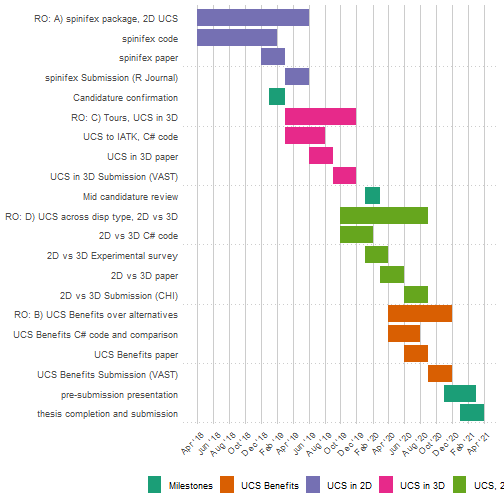
\includegraphics{confirmation_report_ns_files/figure-latex/timeline-1} \end{center}

\emph{Note RO \#2 logically would fit before RO \#3 \& 4, but it is of
lower impact and retrospective performance comparison. I move this
research to the end of the timeline to give the other research
objectives priority in the event of time constraints.}

\section{Accompanying documents}\label{accompanying-documents}

\begin{itemize}
\tightlist
\item
  FIT 5144 hours

  \begin{itemize}
  \tightlist
  \item
    \textgreater{}120 hours \textbf{Tracked, awaiting mandatory events},
    due at the mid-candidature review
  \end{itemize}
\item
  WES Academic record

  \begin{itemize}
  \tightlist
  \item
    FIT6021: 2018 S2, \textbf{Completed} with Distinction
  \item
    FIT5144: 2019 S1+2, \textbf{Upcoming}, due at mid-candidature review
  \item
    FIT5113: 2018 S2, \textbf{Exemption submitted}, forwarded 14/02/2019
  \end{itemize}
\item
  myDevelopment - IT: Monash Doctoral Program - Compulsory Module

  \begin{itemize}
  \tightlist
  \item
    Monash Graduate Research Student Induction: \textbf{Completed}
  \item
    Research Integrity - Choose the Option most relevant:
    \textbf{Completed} (2 required of 4)
  \item
    Faculty Induction: \textbf{Content unavailable} (25/02/2019:
    ``Currently being updated and will be visible in this section
    soon'')
  \end{itemize}
\end{itemize}

\section{Acknowledgements}\label{sec:source}

This report was created in \texttt{R} \autocite{r_core_team_r:_2018},
using \texttt{bookdown} \autocite{xie_bookdown:_2016} and
\texttt{rmarkdown} \autocite{xie_r_2018}, with code generating the
examples inline.

Following best practices of version control, transparency and
reproducibility, the source files can be found at
\href{https://github.com/nspyrison/Confirmation}{github.com/nspyrison/confirmation/}.

\appendix

\chapter{Glossary}\label{ch:glossary}

\section{Tour notation}\label{sec:tour_notation}

Tour notation varies across articles and authors. In my work, I use the
following:

\begin{itemize}
\tightlist
\item
  \(n\), number of observations in the data.
\item
  \(p\), number of numeric variables, the dimensionality of data space.
\item
  \(d\), the dimensionality of projection space.
\item
  \(\textbf{X}_{[n,~p]}\), a data matrix in variable-space,
  \(\textbf{X} \in \mathbb{R}^{p}\). Typically centered, scaled, and
  optionally sphered.
\item
  \(\textbf{B}_{[p,~d]}\), orthonormal (orthogonal and each column
  normalized to a norm of 1) basis set, defining the axes directions for
  the projection from \(p-\) to \(d-\)space.
\item
  \(\textbf{Y}_{[n,~d]}\), projected data matrix in projection-space,
  \(\textbf{Y} \in \mathbb{R}^{d}\).
\item
  Reference axes (or reference frame), a display showing how each
  variables coefficient(s) contribute to a projection. Either on its own
  axis (1D) or relative to a unit circle (2D).
\item
  Geometric objects are referred to in generalized dimensions; the use
  of the term plane is not necessarily a 2D surface, but a hyperplane in
  the arbitrary dimensions of the projection space.
\end{itemize}

\section{Data visualization terminology}\label{sec:3d-terminology}

\begin{itemize}
\tightlist
\item
  2D - representation of data in 2 dimensions, without the use of depth
  perception cues and minimal aesthetic mapping (such as color, size,
  and height) to data points.
\item
  2.5D - following the definition given in
  \textcite{ware_designing_2000}: visualizations that are essentially 2D
  but select depth cues are used to provide some suggestion of 3D.
  However, the term 2.5D is commonly used for several meanings \emph{due
  to the ambiguous use of 2.5D, this document errs on the side stating
  3D with descriptions of depth cues used}.
\item
  3D - visualizations of 3 dimensions with liberal use of depth cues
  unless otherwise qualified.
\item
  Depth perception cues - an indication that indicates the depth to an
  observer, including:

  \begin{itemize}
  \tightlist
  \item
    linear perspective - the property of parallel lines converging on a
    vanishing point.
  \item
    aerial perspective - objects that far away have lower contrast and
    color saturation due to light scattering in the atmosphere.
  \item
    occultation (or interposition) - where closer objects partially
    block the view of further objects.
  \item
    motion perspective/parallax - closer objects, move across the field
    of view faster than further objects.
  \item
    accommodation - the change of focal length due to change in the
    shape of the eye. Effective for distances of less than 2 meters.
  \item
    binocular stereopsis/disparity - the use of 2 images of slightly
    varied angles from the horizontal distance of the eyes. The
    disparity for distant objects is small, but it is significant for
    nearby objects.
  \item
    binocular convergence - The ocular-motor cue due to stereopsis
    focusing on the same objects. Convergence is effective for distances
    up to 10 meters.
  \end{itemize}
\item
  Virtual reality (VR) - an immersive experience of computer-generated
  sensory input.
\item
  Augmented reality (AR) - view of physical spaces with augmenting/
  supplementing sensory input of information.
\item
  Mixed reality (MR) - a mix of physical and virtual realities with
  objects from both interacting in real time. This differs from AR by
  the flow of interaction; AR augments physical reality while MR has
  reciprocating interactions.
\item
  Extended reality (XR) - any degree of virtual, augmented, or mixed
  reality.
\item
  Scatterplot matrices (SPLOMs) - matrix display of pair-wise 2D
  scatterplots, sometimes with 1D density on the diagonal.
\item
  Human-in-the-loop - any model that requires human interaction
  \autocite{karwowski_international_2006}.
\end{itemize}

\chapter{Using animation to explore the sensitivity of structure in a
low-dimensional projection of high-dimensional data with user controlled
steering}\label{ch:spinifex}

\emph{The content contained in this appendix document is work done in
the last year of my research and currently formatted as a paper to be
submitted to the R Journal.}

\section{Abstract}\label{abstract-1}

The class of dynamic linear projections known collectively as tours
provide a unique exploration and feature identification of
high-dimensional data. Tours are particularly useful for understanding
the structure held within multivariate data, and in association with
techniques for dimension reduction, supervised, and unsupervised
classification. The \emph{R} package \emph{tourr} offers a variety of
path generators and geometric displays for conducting tours on. This
paper discusses an extension package, \emph{spinifex}, that adds support
for the path generation of manual tours and graphic display of tours.
Manual tours are used to explore the sensitivity of structure as the
contributions of a manipulation variable are changed. \emph{Spinifex}
utilizes the animation packages \emph{plotly} and \emph{gganimate} to
display tours under animation frameworks.

Keywords: manual tour, guided tour, grand tour, projection pursuit, high
dimensional data, multivariate data, data visualization, statistical
graphics, data science.

\section{Introduction}\label{introduction}

A tour is a multivariate data analysis technique in which a sequence of
linear (orthogonal) projections are viewed as an animation while the
orientation of the projection basis is rotated across time. Each frame
of the sequence corresponds to a small change in the projection for a
smooth transition that perseveres continuity.

There are many ways that a tour path can be generated, we will focus on
the manual tour. The manual tour was described in
\textcite{cook_manual_1997} and allows a user to control the
contribution of a select variable has in the 2D projection. We call such
user-defined manipulation as user-controlled steering (UCS). The primary
purpose of UCS is to determine the sensitivity of structure visible to
the contributions of a selected manipulation variable. This makes UCS
particularly useful once a feature of interest has been identified, for
example, by a guided tour \autocite{cook_grand_1995}. The path of a
guided tour is selected via projection pursuit, the optimization of an
index function on the projection via a hill climbing algorithm. The
algorithm for a manual tour allows rotations in horizontal, vertical,
oblique, angular and radial directions as defined by the values of two
angles. Rotation in a radial direction pulls a variable directly into
and out of the projection. This type of manual rotation illustrated in
this paper.

A manual tour relies on user input and thus has been difficult to
implement dynamic control in R. Ideally, the mouse movements of the user
are captured, and passed to the computations, driving the rotation
interactively. However, this type of interactivity is not simple in R.
This has been the reason that the algorithm was not incorporated into
the \emph{tourr} package. Spinifex utilizes two new animation packages,
\emph{plotly} \autocite{sievert_plotly_2018} and \emph{gganimate}
\autocite{pedersen_gganimate:_2019}, to display tours, manual or other
saved tours. From a given projection, the user can choose which variable
to control, and the animation sequence is generated to remove the
variable from the projection, and then extend its contribution to be the
sole variable in one direction. This allows the viewer to assess the
change in structure induced in the projection by the variable's
contribution.

The paper is organized as follows. Section \ref{sec:algorithm} explains
the algorithm using a toy dataset. Section \ref{sec:display} discussed
the display of the animation after the path has been generated. Section
\ref{sec:application} illustrates how this can be used for sensitivity
analysis applied to contemporary high energy physics. The last section,
\ref{sec:discussion} summarizes the work and discusses future research.

\section{Algorithm}\label{sec:algorithm}

Generating the path for a manual tour requires the iteration of these
steps:

\begin{enumerate}
\def\labelenumi{\arabic{enumi}.}
\tightlist
\item
  Provided with a 2D projection, choose a variable to explore. This is
  called the ``manip'' variable.
\item
  Create a 3D manipulation space, where the manip variable has the full
  contribution.
\item
  Generate a rotation sequence which zero's the norm of the coefficient
  and increases it to 1.
\end{enumerate}

The steps are described in more detail below.

\subsection{Notation}\label{notation}

This section describes the notation used in the algorithm description.
The data is an \(n \times p\) numeric matrix to be embedded into a
\(d-\)dimensions.

\begin{align*}
  \textbf{X}_{[n,~p]} ~=
  \begin{bmatrix}
    X_{1,~1} & \dots  & X_{1,~p} \\
    X_{2,~1} & \dots  & X_{2,~p} \\
    \vdots   & \ddots & \vdots   \\
    X_{n,~1} & \dots  & X_{n,~p}
  \end{bmatrix}
\end{align*}

An orthonormal \(d-\)dimensional basis set is describing the projection
from \(p-\) to \(d-\) space.

\begin{align*}
  \textbf{B}_{[p,~d]} ~=
  \begin{bmatrix}
    B_{1,~1} & \dots  & B_{1,~d} \\
    B_{2,~1} & \dots  & B_{2,~d} \\
    \vdots   & \ddots & \vdots   \\
    B_{p,~1} & \dots  & B_{p,~d}
  \end{bmatrix}
\end{align*}

The algorithm primarily operates on the projection basis and utilizes
the data only when making a display.

\subsection{Toy data set}\label{toy-data-set}

The flea data from \textcite{lubischew_use_1962}, available in the R
package \emph{tourr} \autocite{wickham_tourr_2011}, is used to
illustrate the algorithm. The data contains 74 observations across 6
variables, physical measurements of the flea beetles. Each observation
belonging to one of three species.

A guided tour on the flea data is conducted by optimizing on the
\texttt{holes} index \autocite{cook_interactive_2007}. In a guided tour
the projection sequence is selected by optimizing an index of interest.
In this case, the holes index is selected. The holes index is maximized
by when the projected observations are furthest from the center. Figure
\ref{fig:step0}, shows a locally optimized projection for this data. The
left plot displays the reference axes of the projection basis, a visual
indication of the magnitude and direction each variable contributed to
the projections. The right plot shows the data projected through this
basis. The variables \texttt{tars1} and \texttt{aede2} contribute mostly
in the horizontal direction mostly orthogonal to the other four
variables which explain more of the variation in the verticle direction
of the projection. Data points are colored and given geoms according to
the species of the flea, although the guided tour was unsupervised with
this information. The question that will be explored in the explanation
of the algorithm is how important is the variable \texttt{aede2} to the
separation of the clusters.

\begin{figure}

{\centering 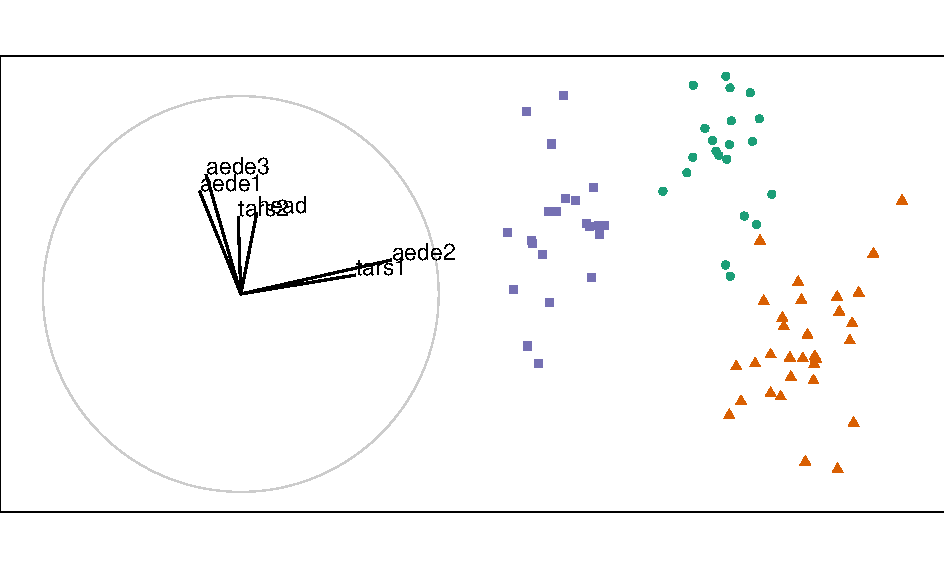
\includegraphics[width=0.98\linewidth]{confirmation_report_ns_files/figure-latex/step0-1} 

}

\caption{Basis reference axes (left) and projected data (right) of standardized flea data. Basis identified by holes-index guided tour. The variables `aede2` and `tars1` contribute mostly in the horizontal direction, whereas the other variables contribute mostly in the y direction. We'll select `aede2` as our manipulation variable to see how the structure of the projection changes as we rotate `aede2` into and out of the projection.}\label{fig:step0}
\end{figure}

Call \texttt{view\_basis()} on a basis to produce a similar image as a
\texttt{ggplot2} object. The right side shows how the data looks
projected through this basis. If data is passed to the function, the
projection will also be displayed. You can project a single basis at any
time through the matrix multiplication
\(\textbf{X}_{[n,~p]} ~*~ \textbf{B}_{[p,~d]} ~=~ \textbf{P}_{[n,~d]}\)
to this effect.

\subsection{Step 1 Choose variable of
interest}\label{step-1-choose-variable-of-interest-1}

Select a manipulation variable, \(k\). Initialize a zero vector \(e\)
and set the \(k\)-th element set to 1. This gives the manip variable
full contribution in this dimension.

\begin{align*}
\textbf{e}_{[p,~1]} ~=~
  \begin{bmatrix}
    0 \\
    0 \\
    \vdots \\
    1 \\
    \vdots \\
    0
  \end{bmatrix}
\end{align*}

In figure \ref{fig:step0}, above, notice that the variables
\texttt{tars1} and \texttt{aede2} are almost orthogonal to the other 4
variables and control almost all of the variation in the x-axis of the
projection. \texttt{Aede2} has a larger contribution on this basis, so
we'll select it as the manip variable.

\subsection{Step 2 Create the manip
space}\label{step-2-create-the-manip-space-1}

Use the Gram-Schmidt process to orthonormalize the concatenation of the
basis and \(e\) yielding the manipulation space.

\begin{align*}
  \textbf{M}_{[p,~d+1]}
  &= Orthonormalize_{GS}( \textbf{B}_{[p,~d]}|\textbf{e}_{[p,~1]} ) \\
  &= Orthonormalize_{GS}
  \left(
    \begin{bmatrix}
      B_{1,~1} & \dots  & B_{1,~d} \\
      B_{2,~1} & \dots  & B_{2,~d} \\
      \vdots   & \ddots & \vdots   \\
      B_{k,~1} & \dots  & B_{k,~d} \\
      \vdots   & \ddots & \vdots   \\
      B_{p,~1} & \dots  & B_{p,~d}
    \end{bmatrix}
  ~|~
    \begin{bmatrix}
      0 \\
      0 \\
      \vdots \\
      1 \\
      \vdots \\
      0
    \end{bmatrix}
  \right)
\end{align*}

Adding an extra dimension to our basis plane allows for the manipulation
of the specified variable. For example, lifting a piece of paper, rather
than manipulating on a table top. Orthonormalizing rescales the new
vector while leaving the first \(d\) variables identical to the basis.
An illustration of such can be seen below in figure \ref{fig:step2}.

\begin{figure}

{\centering 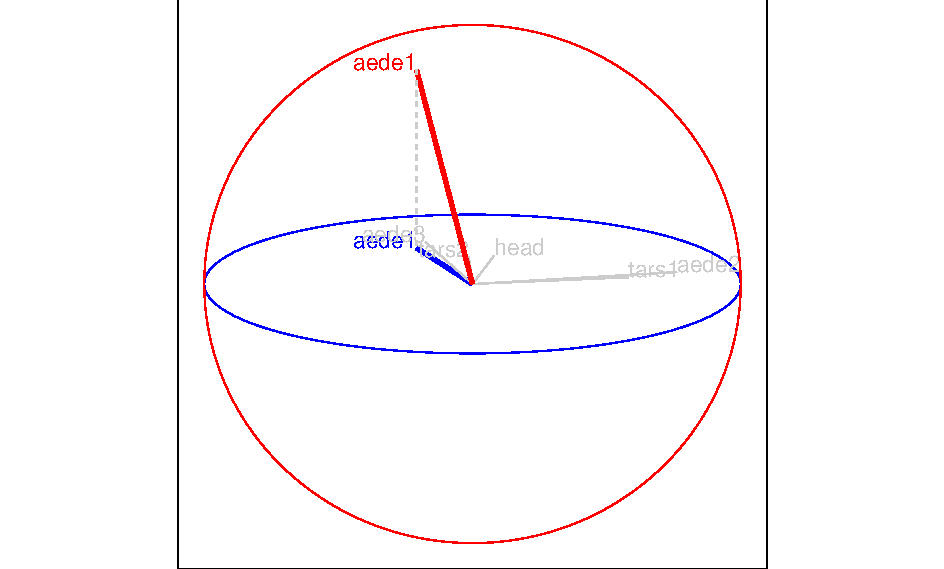
\includegraphics[width=1\linewidth]{confirmation_report_ns_files/figure-latex/step2-1} 

}

\caption{Manipulation space for controlling the contribution of aede2 of standardized flea data. Basis was identified by holes-index guided tour. The out of plane axis, in red, shows how the manipulation variable can be rotated, while other dimensions stay embedded within the basis plane.}\label{fig:step2}
\end{figure}

Imagine being able to grab hold of the red axis and rotate it changing
the projection onto the basis plane. This is what happens in a manual
tour. For a radial tour, fix \(\phi\), the angle within the blue plane,
and vary the \(\theta\), the angle between the red and blue lines. The
user controlling these angles changes the values of the coefficient the
manip variable and performs a constrained rotation on the remaining
variables.

\subsection{Step 3 Generate rotation}\label{step-3-generate-rotation-1}

Define a set of values for \(\phi_i\), the angle of out of the plane
rotation, orthogonal to the projection plane. This corresponds to the
angle between the red manipulation axis and the blue plane in figure
\ref{fig:step2}.

\textbf{For } \(i\) \textbf{in 1 to n\_slides:}

Post-multiply the manipulation space by a rotation matrix, producing,
\textbf{RM}, the rotated manip space.

\begin{align*}
  \textbf{RM}_{[p,~d+1,~i]}
  &= \textbf{M}_{[p,~d+1]} ~*~ \textbf{R}_{[d+1,~d+1]}
    ~~~~~~~~~~~~~~~~~~~~~~~~\text{For the $d=2$ case:} \\
  &= \begin{bmatrix}
    M_{1,~1} & \dots & M_{1,~d} & M_{1,~d+1} \\
    M_{2,~1} & \dots & M_{2,~d} & M_{2,~d+1} \\
    \vdots   & \ddots& \vdots   \\
    M_{p,~1} & \dots & M_{p,~d} & M_{p,~d+1}
  \end{bmatrix}_{[p,~d+1]}
    ~*~
  \begin{bmatrix}
    c_\theta^2 c_\phi s_\theta^2 &
    -c_\theta s_\theta (1 - c_\phi) &
    -c_\theta s_\phi \\
    -c_\theta s_\theta (1 - c_\phi) &
    s_\theta^2 c_\phi + c_\theta^2 &
    -s_\theta s_\phi \\
    c_\theta s_\phi &
    s_\theta s_\phi &
    c_\phi
  \end{bmatrix}_{[3,~3]}
\end{align*}

Where:

\begin{description}
  \item[$\theta$] is the angle that lies on the projection plane, the *XY*-scatterplot
  \item[$\phi$] is the angle orthogonal to the projection plane, in the *Z* direction relative to the *XY*-scatterplot
  \item[$c_\theta$] is the cosine of $\theta$
  \item[$c_\phi$]   is the cosine of $\phi$
  \item[$s_\theta$] is the sine of   $\theta$
  \item[$s_\phi$]   is the sine of   $\phi$
\end{description}

In application: compile the sequence of \(\phi_i\) and create an array
(or long table) for each rotated manipulation space. \(\phi\) is the
angle relative to the initial value of \(\phi\), we find the
transformation \(\phi_i\) - \(\phi_1\) useful to think about \(\phi\)
relative to the basis plane. If the manip variable doesn't move as
expected this is the first place to check.

\begin{Shaded}
\begin{Highlighting}[]
\ControlFlowTok{for}\NormalTok{ (phi }\ControlFlowTok{in} \KeywordTok{seq}\NormalTok{(seq_start, seq_end, phi_inc_sign)) \{}
\NormalTok{  slide <-}\StringTok{ }\NormalTok{slide }\OperatorTok{+}\StringTok{ }\DecValTok{1}
\NormalTok{  tour[,, slide] <-}\StringTok{ }\KeywordTok{rotate_manip_space}\NormalTok{(manip_space, theta, phi)[, }\DecValTok{1}\OperatorTok{:}\DecValTok{2}\NormalTok{]}
\NormalTok{\}}
\end{Highlighting}
\end{Shaded}

In figure \ref{fig:step3} we illustrate the sequence with 15 projected
bases and highlight the manip variable on top while showing the
corresponding projected data points on the bottom. A dynamic version of
this tour can be viewed online at
\url{https://nspyrison.netlify.com/thesis/flea_manualtour_mvar5/}, which
may take a moment to load. The format of this figure and linking to a
dynamic version will be used again in section \ref{sec:application}.









\begin{figure}

{\centering 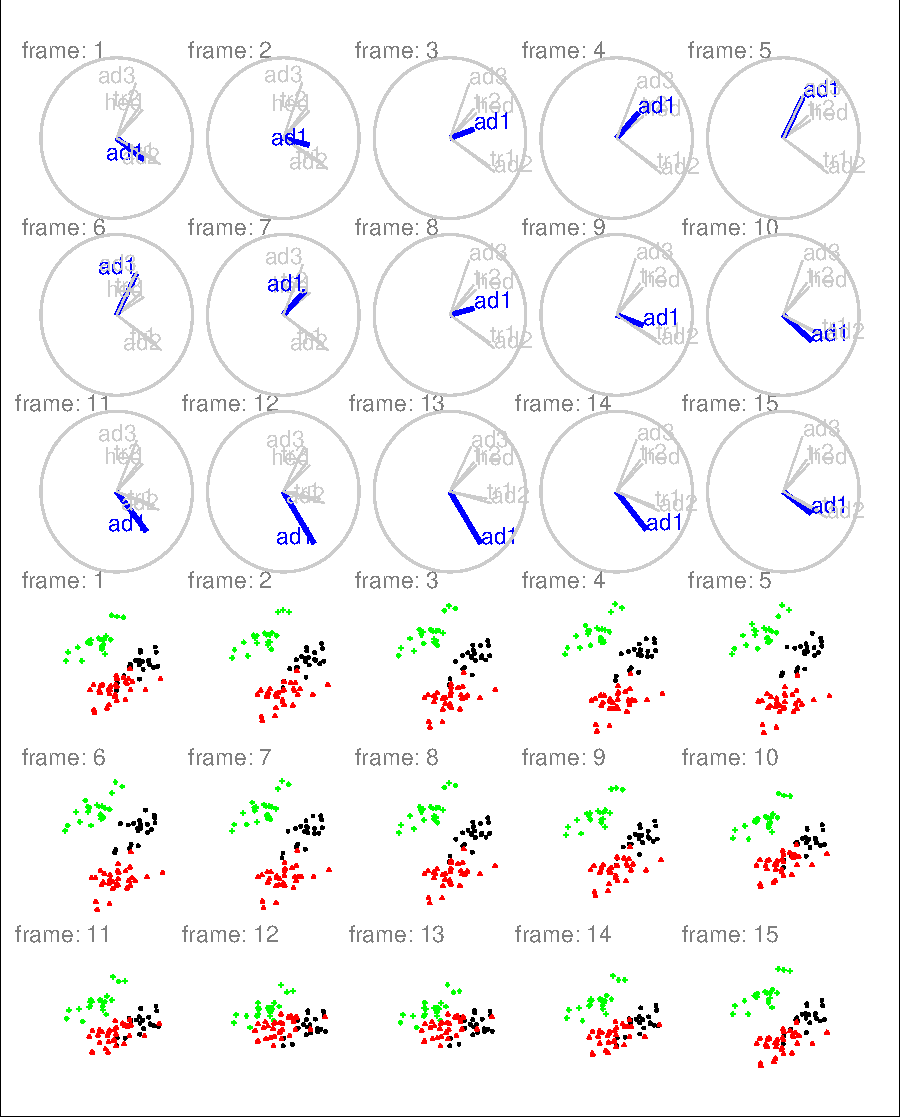
\includegraphics[width=6in,height=7.2in]{confirmation_report_ns_files/figure-latex/step3-1} 

}

\caption{Rotated manipulation spaces, a radial manual tour
controlling the contribution from \texttt{aded2} of standardized flea
data. The contribution of \texttt{aede2} extends from its initial
contribution to a full contribution to the projection before decreasing
to zero and then returning to its initial value. A dynamic version can
be viewed at
\url{https://nspyrison.netlify.com/thesis/flea_manualtour_mvar5/}.}\label{fig:step3}
\end{figure}

\section{Display projection sequence}\label{sec:display}

To get back to data-space pre-multiply each rotated manip space by the
data for the projection in data-space.

\begin{align}
  \textbf{P}_{[n,~d+1]}
    &= \textbf{X}_{[n,~p]} ~*~ \textbf{RM}_{[p,~d+1]} \\
    &=
      \begin{bmatrix}
          X_{1,~1} & \dots & X_{1,~p} \\
          X_{2,~1} & \dots & X_{2,~p} \\
          \vdots   & \vdots & \vdots  \\
          X_{n,~1} & \dots & X_{n,~p}
      \end{bmatrix}_{[n,~p]}
      ~*~
      \begin{bmatrix}
        RM_{1,~1} & RM_{1,~2} & RM_{1,~3} \\
        RM_{2,~1} & RM_{2,~2} & RM_{2,~3} \\
        \vdots     & \vdots     & \vdots     \\
        RM_{p,~1} & RM_{p,~2} & RM_{p,~3}
      \end{bmatrix}_{[p,~d+1]}
\end{align}

Plot the first 2 variables from each projection in sequence for an
\(XY\) scatterplot. The remaining variable is sometimes linked to a data
point aesthetic to produce depth cues used in conjunction with the
\(XY\) scatterplot.

\emph{tourr} utilizes R's base graphics for the display of tours. Use
\texttt{render\_plotly()} to display as an dynamic \texttt{plotly}
\textcite{sievert_plotly_2018} object or \texttt{render\_gganimate()}
for a \texttt{gganimate} \textcite{pedersen_gganimate:_2019} graphic.
Both of which build off of \texttt{ggplot2} plotting in internal
functions.

Interaction with graphics in R is limited. Traditionally, all commands
are passed to the R via calls to the console, conflicting with user
engagement. Some recent packages have made advancement into this
direction such as with the use of the R package \texttt{shiny}
\autocite{chang_shiny:_2018}, which allows applications can be hosted
either locally or remotely and communicate with the R console, allowing
for developers to code dynamic content interaction. To a lesser extent,
\texttt{plotly} offers static interactions with the contained object,
such as tooltips, brushing, and linking without communicating back to
the R console.

\subsection{Storage and sharing}\label{storage-and-sharing}

Storing each data point for every frame of the animation is very
inefficient. In the same way that we gain efficiency by performing math
on the bases, that is the same approach suggested for storage and
sharing tours. Consider a radial manual tour, we can store the salient
features in 3 bases, where \(\phi\) is at its starting, minimum, and
maximum values. The frames in between can be interpolated by supplying
angular speed. By using the function \texttt{tourr::save\_history()} we
can do just that. Save such tour path history and a single set of data
offers performant storage and transfer.

\section{Application}\label{sec:application}

In a recent paper, \textcite{wang_visualizing_2018}, the authors
aggregate and visualize the sensitivity of hadronic experiments, in the
field of high energy physics. The authors introduce a new tool,
PDFSense, to aid in the visualization of parton distribution functions
(PDF). The parameter-space of these experiments lies in 56 dimensions,
\(\delta \in \mathbb{R}^{56}\), and are presented in as 2D subspaces of
the 6 and 10 first principal components in linear and non-linear
embeddings.

The work in \textcite{cook_dynamical_2018} applies manual tours to
discern the finer structure of this sensitivity. Table 1 of Cook et. al.
summaries the key findings of PDFSense \& TFEP (TensorFlow embedded
projections) and those from manual tours. The authors selected the 6
first principal components, containing 48\% of the variation held within
the full data when centered, but not sphered. This data contained 3
clusters: jet, DIS, and VBP. The initial basis sets used below are
obtained from projections used in figures 7 and 8 of the previous study
(jet and DIS clusters respectively) of the previous study and apply
manual tours to explore the local structure with finer precision.

\subsection{Jet cluster}\label{jet-cluster}

The jet cluster is of particular interest as it contains the largest
data sets and is found to be important in
\textcite{wang_visualizing_2018}. The jet cluster resides in a smaller
dimensionality than the full set of experiments with 4 principal
components explaining 95\% of its variation
\autocite{cook_dynamical_2018}. We subset the data down to ATLAS7old and
ATLAS7new to narrow in on 2 groups with a reasonable number of
observations and occupy different parts of the subspace. Below, we
perform radial manual tours on various principal components within this
scope. In PC3 and PC4 are manipulated in figure \ref{fig:JetClusterGood}
and figure \ref{fig:JetClusterBad} respectively. Manipulating PC3, where
varying the angle of rotation brings interesting features into and out
of the center mass of the data, is more interesting than the
manipulation of PC4, where the features are mostly independent of the
contribution of PC4.










\begin{figure}

{\centering 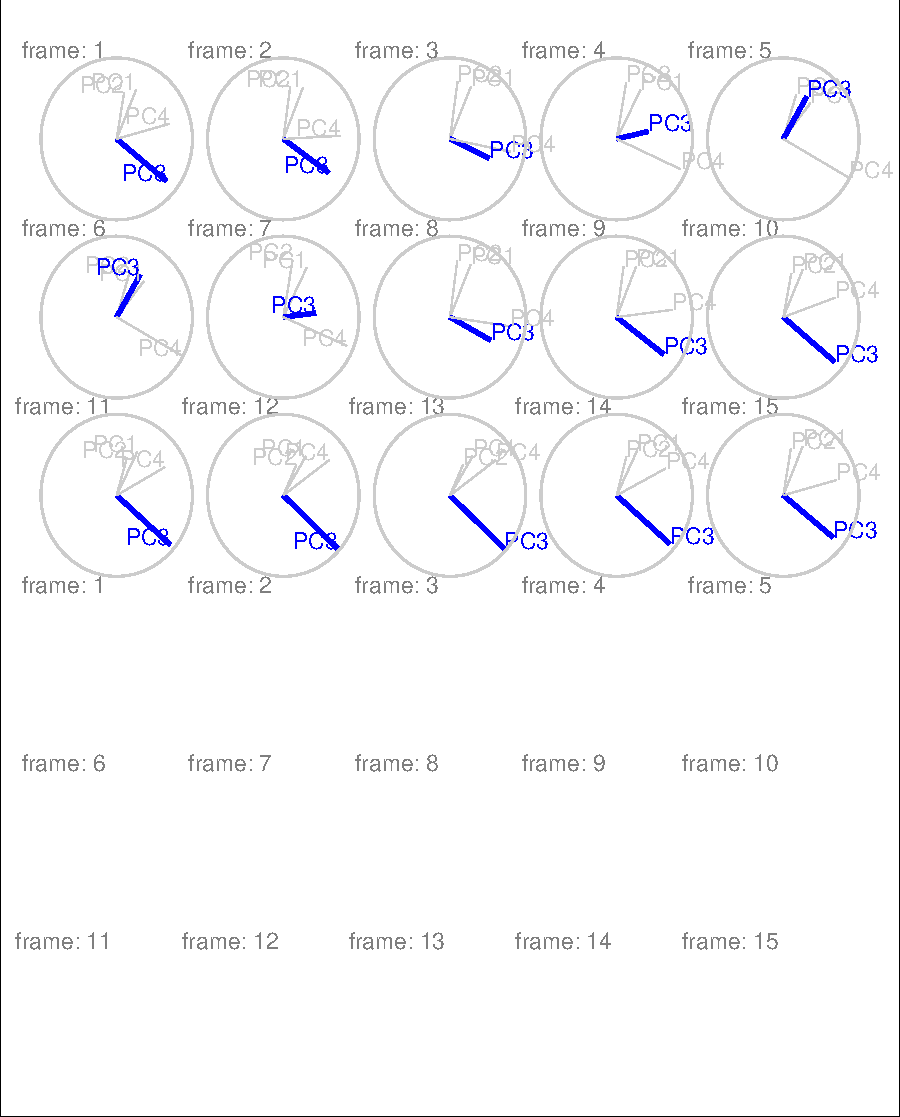
\includegraphics[width=6in,height=7.2in]{confirmation_report_ns_files/figure-latex/JetClusterGood-1} 

}

\caption{Jet cluster, a radial manual tour of PC3.
Colored by experiment type: `ATLAS7new' in green and `ATLAS7old' in
orange. When PC3 fully contributes to the projection ATLAS7new (green)
occupies unique space and several outliers are identifiable. Zeroing the
contribution from PC3 to the projection hides the outliers and indeed
all observations with ATLAS7new are contained within ATLAS7old (orange).
A dynamic version can be viewed at
\url{https://nspyrison.netlify.com/thesis/jetcluster_manualtour_pc3/}.}\label{fig:JetClusterGood}
\end{figure}









\begin{figure}

{\centering 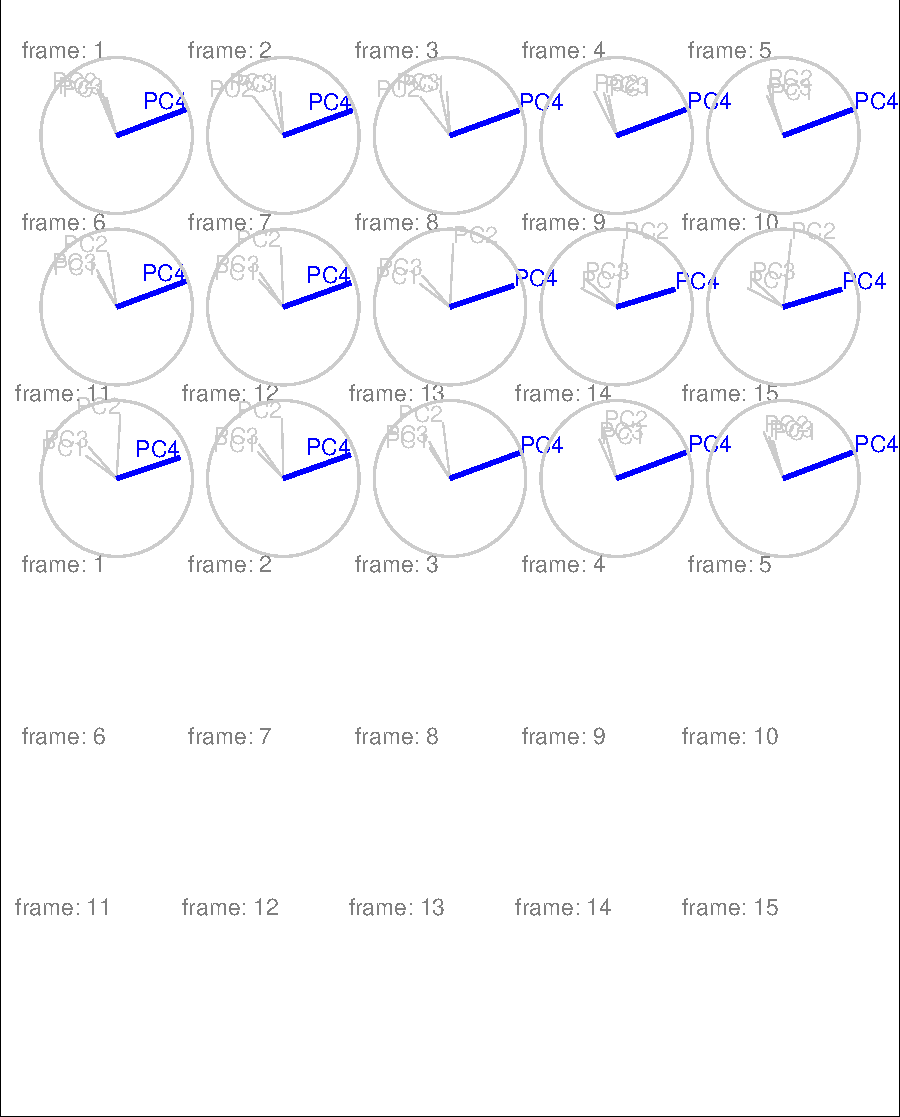
\includegraphics[width=6in,height=7.2in]{confirmation_report_ns_files/figure-latex/JetClusterBad-1} 

}

\caption{Jet cluster, a radial manual tour of PC4.
Colored by experiment type: `ATLAS7new' in green and `ATLAS7old' in
orange. This tour contains less interesting information ATLAS7new
(green) has points that are right and left of ATLAS7old, while most
points occupy the same projection space, regardless of the contribution
of PC4. A dynamic version can be viewed at
\url{https://nspyrison.netlify.com/thesis/jetcluster_manualtour_pc3/}.}\label{fig:JetClusterBad}
\end{figure}

Jet cluster manual tours manipulating each of the principal components
can be viewed from the links:
\href{https://nspyrison.netlify.com/thesis/jetcluster_manualtour_pc1/}{PC1},
\href{https://nspyrison.netlify.com/thesis/jetcluster_manualtour_pc2/}{PC2},
\href{https://nspyrison.netlify.com/thesis/jetcluster_manualtour_pc3/}{PC3},
and
\href{https://nspyrison.netlify.com/thesis/jetcluster_manualtour_pc4/}{PC4}.

\subsection{DIS cluster}\label{dis-cluster}

We perform a manual tour on this data, manipulating PC6 as depicted in
figure \ref{fig:DISclusterGood}. Looking at several frames we see that
DIS HERA data lies mostly on a plane. When PC6 has full contributions,
we see the dimuon SIDIS in purple is almost orthogonal to the DIS HERA
(green). Yet the contribution of PC6 has zeroed the dimuon SIDIS data
occupy the same space as the DIS HERA data. A dynamic version of this
manual tour can be found at:
\url{https://nspyrison.netlify.com/thesis/discluster_manualtour_pc6/}.
The page may some time to load, as the animation is several megabytes.











\begin{figure}

{\centering 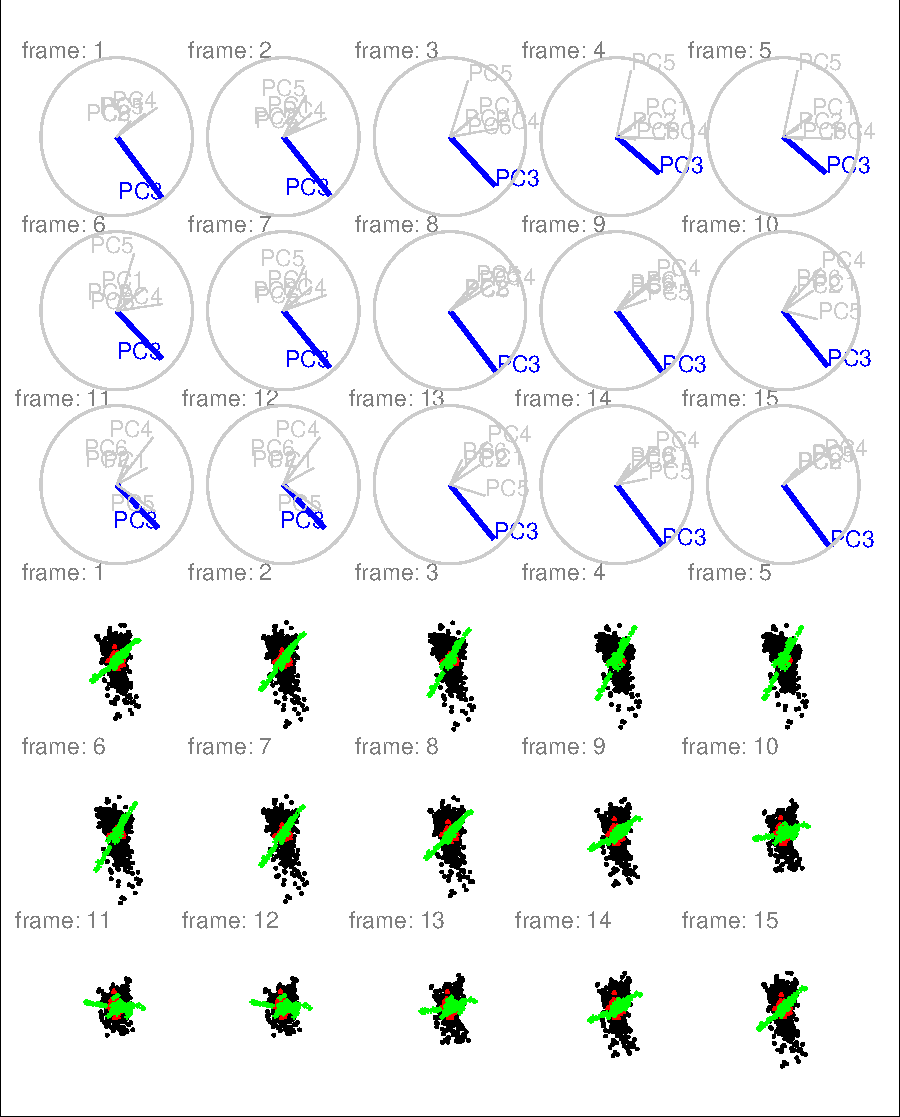
\includegraphics[width=6in,height=7.2in]{confirmation_report_ns_files/figure-latex/DISclusterGood-1} 

}

\caption{DIS cluster, a radial manual tour of PC6.
colored by experiment type: `DIS HERA1+2' in green, `dimuon SIDIS' in
purple, and `charm SIDIS' in orange. When the contribution PC 6 is large
we see that dimuon SIDIS (purple) data are nearly orthogonal to DIS HERA
(green) data. As the projection is rotated, we can also see that DIS
HERA (green) practically lies on a plane in this 6-d subspace. When the
contribution of PC6 is near zero, dimonSIDIS (purple) occupies the same
space as the DIS HERA data. A dynamic version can be viewed at
\url{https://nspyrison.netlify.com/thesis/discluster_manualtour_pc6/}.}\label{fig:DISclusterGood}
\end{figure}

The selection of the correct manip variable is important as the
manipulation spaces convey different information. For example, in figure
\ref{fig:DISclusterBad} we select PC2 as the manip variable finding it
to be less insightful than PC6.










\begin{figure}

{\centering 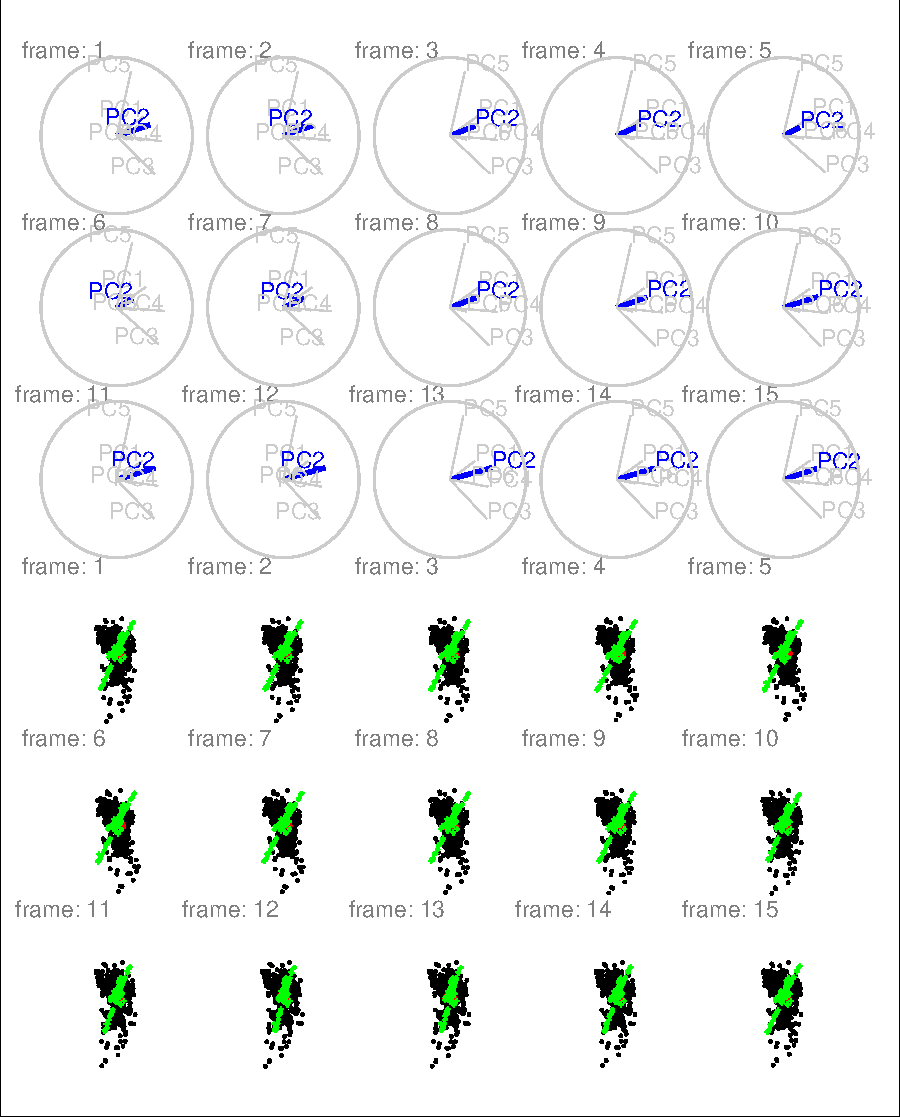
\includegraphics[width=6in,height=7.2in]{confirmation_report_ns_files/figure-latex/DISclusterBad-1} 

}

\caption{DIS cluster, a radial manual tour of PC2.
Colored by experiment type: `DIS HERA1+2' in green, `dimuon SIDIS' in
purple, and `charm SIDIS' in orange. The structure of previously
described plane of DIS HERA (green) and nearly orthogonal dimuon SIDIS
(purple) is present, however, the manipulating PC2 does not give a
head-on view of either, a less useful manual tour than that of PC6. A
dynamic version can be viewed at
\url{https://nspyrison.netlify.com/thesis/discluster_manualtour_pc2/}.}\label{fig:DISclusterBad}
\end{figure}

DIS cluster manual tours manipulating each of the principal components
can be viewed from the links:
\href{https://nspyrison.netlify.com/thesis/discluster_manualtour_pc1/}{PC1},
\href{https://nspyrison.netlify.com/thesis/discluster_manualtour_pc2/}{PC2},
\href{https://nspyrison.netlify.com/thesis/discluster_manualtour_pc3/}{PC3},
\href{https://nspyrison.netlify.com/thesis/discluster_manualtour_pc4/}{PC4},
\href{https://nspyrison.netlify.com/thesis/discluster_manualtour_pc5/}{PC5},
and
\href{https://nspyrison.netlify.com/thesis/discluster_manualtour_pc6/}{PC6}.

\section{Source code and usage}\label{source-code-and-usage}

This article was created in \texttt{R} \autocite{r_core_team_r:_2018},
using \texttt{bookdown} \autocite{xie_bookdown:_2016} and
\texttt{rmarkdown} \autocite{xie_r_2018}, with code generating the
examples inline. The source files can be found at
\href{https://github.com/nspyrison/confirmation/}{github.com/nspyrison/confirmation/}.

The source code for the \texttt{spinifex} package can be found at
\href{https://github.com/nspyrison/spinifex/}{github.com/nspyrison/spinifex/}.
To install the package in R, run:

\begin{Shaded}
\begin{Highlighting}[]
\CommentTok{# install.package("devtools")}
\NormalTok{devtools}\OperatorTok{::}\KeywordTok{install_github}\NormalTok{(}\StringTok{"nspyrison/spinifex"}\NormalTok{)}
\end{Highlighting}
\end{Shaded}

\section{Discussion}\label{sec:discussion}

This research has modified the algorithm producing manual tours in
extends animations of tours to other graphics packages. Tour paths
generated in \texttt{tourr} can also be viewed using these frameworks.

Future research on the algorithm would include extending it for use in
3D projections. This would allow for projections in immersive virtual
reality, which may allow for a better perception of structure and enable
function visualization. The \texttt{tourr} package provides many other
geometric displays with the \texttt{tourr::display\_*()} family. These
other geoms should be integrated into the \texttt{ggplot2} framework for
display on \texttt{plotly} and \texttt{gganimate}.

The Givens rotations and Householder reflections as outlined in
\textcite{buja_computational_2005} could also be added. Currently,
Gram-Schmidt is the only form of frame interpolation used. In a Givens
rotation, the \(x\) and \(y\) components (for example
\(\theta~= 0,~pi/2\)) of the in-plane rotation are calculated separately
and would be applied sequentially to produce the radial rotation.
Householder reflections define reflection axes to project points on to
the axes and generate rotations.

The development of a dynamic graphical user interface, perhaps with the
use of a \texttt{shiny} app, would allow analysts to rapidly try manual
tours with a more intuitive interaction than the command line. The user
could easily switch between variables to control, adjust the step size
to make smoother rotation sequences, or save any state to continue to
explore the contributions of other variables. The \texttt{animation}
package \textcite{xie_animation:_2018} could be implemented for another
graphics framework. However, \texttt{animation} builds from base graphs
while \texttt{spinifex} current utilizes \texttt{ggplot2} graphics.

\printbibliography[heading=bibintoc]



\end{document}
